\documentclass[conference]{IEEEtran}
\IEEEoverridecommandlockouts
% The preceding line is only needed to identify funding in the first footnote. If that is unneeded, please comment it out.

% test
\usepackage{amsmath,amssymb,amsfonts}
\usepackage{algorithmic}
\usepackage{graphicx}
\usepackage{textcomp}
\usepackage{xcolor}
\usepackage{lscape}
\usepackage{float}
\usepackage{multirow}
\usepackage{tcolorbox}
\usepackage{booktabs}
\usepackage{caption}
\usepackage{subcaption}
\usepackage{url}
\usepackage{balance}
\usepackage[numbers, sort]{natbib}
\def\BibTeX{{\rm B\kern-.05em{\sc i\kern-.025em b}\kern-.08em
		T\kern-.1667em\lower.7ex\hbox{E}\kern-.125emX}}
\usepackage[colorlinks = true,
            linkcolor = black,
            urlcolor  = blue,
            citecolor = black,
            anchorcolor = black]{hyperref}
            
\newcommand{\boxedtext}[1]{\fbox{\scriptsize\bfseries\textsf{#1}}}
\newcommand{\nota}[2]{
	\boxedtext{#1}
	{\small$\blacktriangleright$\emph{\textsl{#2}}$\blacktriangleleft$}
}

\newcommand{\FIXME}[1]{{\color{red}\textsf{FIXME: #1}}}
\newcommand{\todo}[1]{{\color{red}\nota{TODO}{#1}}}
\newcommand{\fix}[1]{\textcolor{blue}{#1}}

\definecolor{lightblue}{RGB}{32, 209, 228}
\definecolor{darkgreen}{RGB}{0, 64, 0}
\definecolor{darkyellow}{RGB}{255, 204, 0}

\begin{document}
	
	\title{Achilles: Prioritizing Vulnerable Dependency Updates through Dependency Graphs}
	
	\author{\IEEEauthorblockN{Vipawan Jarukitpipat\textsuperscript{\textasteriskcentered}, Klinton Chhun\textsuperscript{\textasteriskcentered},
			Wachirayana Wanprasert\textsuperscript{\textasteriskcentered},
			Chaiyong Ragkhitwetsagul\textsuperscript{\textasteriskcentered}, \\
			Raula Gaikovina Kula\textsuperscript{\textdagger},
			Bodin Chinthanet\textsuperscript{\textdagger},
			Takashi Ishio\textsuperscript{\textdagger}, \\
			Morakot Choetkiertikul\textsuperscript{\textasteriskcentered}, 
			Thanwadee Sunetnanta\textsuperscript{\textasteriskcentered},
			Kenichi Matsumoto\textsuperscript{\textdagger}
		}
		\IEEEauthorblockA{\textsuperscript{\textasteriskcentered}\textit{Faculty of Information and Communication Technology (ICT), Mahidol University, Thailand} \\
			\textsuperscript{\textdagger}\textit{Nara Institute of Science and Technology (NAIST), Japan}\\
			\textit{Email: \{vipawan.jau, wachirayana.wan, klinton.chh}@student.mahidol.edu\}\\ 
			\textit{\{raula-k, bodin.chinthanet.ay1, ishio, matumoto\}@is.naist.jp},
			\textit{\{chaiyong.rag, morakot.cho, thanwadee.sun\}@mahidol.edu}
		}
	}
	\maketitle
	\thispagestyle{plain}
	\pagestyle{plain}
	
	\begin{abstract}
		The use of third-party dependencies in software applications is commonplace for contemporary software development, especially with the rise of available software library ecosystems like the Node.js packages (npm). 
		A key threat to the usage of third-party dependencies has been the threat of security vulnerabilities, which risks unwanted access to a user application. 
		As part of an ecosystem of dependencies, users of a library are prone to both the direct and indirect (transitives) dependencies that they have adopted into their application. 
		Recent work involves tool support for vulnerable dependency updates, but the extent to which these tools aid the prioritization of dependency updates is unknown. 
		In this paper, we adopt a visual approach to understand how to prioritize a vulnerable dependency update.
		As a prototype, we present \texttt{Achilles}, which is a tool that shows a visualization (i.e., using dependency graphs) of complexity of dependencies and both direct and indirect dependencies that are affected by vulnerability attacks.
		To evaluate the effectiveness of \texttt{Achilles}, we conducted a user study with 20 participants against the state of the art tools (Dependabot and npm audit).
		We found that 7 out of the 10 participants exposed to Achilles re-prioritized their updates, which is much higher than the other tools.
		We show that there is a difference in using a visualization, complexity of the dependency and indirect dependencies are factors that developers consider. 
		Our prototype is available for usage at \url{https://github.com/MUICT-SERU/Achilles}.
	\end{abstract}
	
	\begin{IEEEkeywords}
		software libraries, fixing known vulnerabilities, dependency graph, software visualization
	\end{IEEEkeywords}
	
	\section{Introduction}
	The use of third-party dependencies in software applications is now prevalent for contemporary software development. 
	Much of this is due to the rise of available software library ecosystems like the Node.js packages (npm), which now hosts over 1.6 million library packages and is relied upon by more than 11 million developers worldwide\footnote{\url{https://www.npmjs.com/}}.
	Furthermore, the importance of npm packages is evident in industry, by its purchased by Microsoft's GitHub in 2020\footnote{\url{https://github.blog/2020-03-16-npm-is-joining-github/}}.
	
	A key threat to the usage of third-party dependencies has been security vulnerabilities, which risks unwanted access to a user application. 
	Furthermore, as part of an ecosystem of dependencies, users of a library is prone to both the direct and indirect (transitives) dependencies that they have adopted into their application \citep{Kikas:2017, Decan:2018, Chinthanet2021}. 
	The typical response to security vulnerability is a security advisory, which lets developers know of the security threats. 
	For instance, the GitHub Advisory Database (GHSA)\footnote{\url{https://github.com/advisories}} contains a curated list of security vulnerabilities that have been mapped to packages tracked by the GitHub and stored in the Common Vulnerabilities and Exposures (CVE) format along with the type of software weaknesses that they belong to (CWE). 
	The GHSA is sourced from the National Vulnerability Database (NVD)\footnote{\url{https://nvd.nist.gov/}} and the npm security advisories.\footnote{\url{https://www.npmjs.com/advisories}}
	
	Together with security advisories, there has been recent work that involve tool support for vulnerable dependency updates.
	Two tools that have been prevalent and the state of the art is both Dependabot \cite{Web:github_dependabot} and npm audit \cite{Web:npm_audit}. 
	Both tools help developers, by identifying vulnerabilities in existing dependencies. 
	Dependabot actually automatically creates a pull request to update the dependencies. 
	Recent work from \citet{Alfadel:MSR2021} found that developers are highly receptive to pull requests from Dependabot.
	However, even with these tools, developers struggle to update their dependencies. 
	Prior studies showed that developers are slow in updating their dependencies \citep{Robbes:2012, Hora:2015, Sawant2016, Bavota:2015, Ihara:2017} due to various factors such as compatibility issues, being unaware, and the migration effort outweighing the benefits.
	Other work \cite{Kula2018} similarly find that most developers were unaware of dependency updates, and also cited other issues such as the migration effort as a barrier to adopting a dependency update.
	We posit that given more information, \textit{developers may re-prioritize their decisions to update}, hence may relate to evaluating the migration effort needed to update. 
	Although tools exist to provide a fix, the extent to which developers prioritize which security updates should be fixed is still unknown.
	
	In this paper, we adopt a visual approach to understand how developers can use more dependency information to prioritize their decisions on which vulnerable dependency to update \citep{Chen:VISSOFT2020}. 
	As a prototype, we present \texttt{Achilles}, which is a tool that shows a visualization (i.e., using dependency graphs) of both direct and indirect dependencies that are affected by software vulnerability attacks.
	To evaluate the effectiveness of \texttt{Achilles}, we performed a user study against the state-of-the-art tools (Dependabot and npm audit). 
	We recruited twenty participants to perform two tasks of prioritizing dependency vulnerabilities to fix. For Task 1, we found that seven out of ten participants who used \texttt{Achilles} gave different prioritization from when using Dependabot report compared to four participants who used npm audit. For Task 2, we similarly found that seven out of ten \texttt{Achilles} participants gave different prioritization from when using Dependabot report compared to six participants who used npm audit.
	We also found that the participants who used npm audit re-prioritized their dependency updates after introduced to \texttt{Achilles}.
	
	Results show that the graph visualization of \texttt{Achilles} helps supporting developers' decisions on prioritizing vulnerability to fix by providing more information about complexity and indirect dependencies. Furthermore, we show that a dependency graph visualization is more effective at re-prioritizing developers decisions when showing complexity of the dependency, as opposed to the indirect vulnerability dependencies.
	Our work shows that  visual tool support is needed for prioritizing dependency updates.
	
	\section{Background and Basic Concepts}
	In this section, we show the list of prior works and key concepts related to dependencies, issues on dependency updating, and security vulnerabilities.
	
	%\subsection{Library Dependencies}
	%In contemporary software development, using third-party libraries or dependencies is a common practice. The developers can easily incorporate a new dependency into their software project with only a single statement. This activity reduces the developers' effort in writing code from scratch and also avoid repeating steps in software development for such code including designing, writing, testing, debugging, and maintaining a specific unit of code~\cite{Cox2019}.
	
	\subsection{Direct vs.~Indirect Dependencies}
	A \textit{direct dependency} means a software dependency that is directly called from the developer's code. This type of dependencies are found in \texttt{include} or \texttt{import} statements or in a dependency file such as \texttt{package.json}. The direct dependencies usually contains functionalities that the developer wants to include in their software project and the calls to such functionalities can be found in the project code. 
	
	On the other hand, an \textit{indirect dependency} or \textit{transitive dependency} is a software dependency that is called from another dependency (either direct or indirect dependency). Similar to the direct dependency, the indirect dependencies contain functionalities that the other dependencies require or depend on. The indirect dependencies can be created in different levels depending on how many dependency calls occur. A thread of all the dependencies that depend on each other from the project to the dependency in the last level can be called a \textit{chain of dependencies}. For example, in an npm project \texttt{P}, the project has a direct dependency called \texttt{karma-mocha}. This direct dependency depends on another dependency called \texttt{minimist}. This creates a chain of dependencies of \texttt{P} $\rightarrow$ \texttt{karma-mocha} $\rightarrow$ \texttt{minimist}.
	One direct dependency can create several indirect dependencies by calling several other dependencies in their code. Previous study~\cite{Zimmermann2019} shows that there are approximately 80 indirect dependencies per one direct dependency installed and this ratio is increasing over time. This large number of indirect dependencies and their invisibility from the developer's point of view can result in difficulty in locating flaws or vulnerabilities introduced to the software project by the indirect dependencies~\cite{Cox2019,Snyk2020}.
	
	\begin{figure*}[!tb]
		\centering
		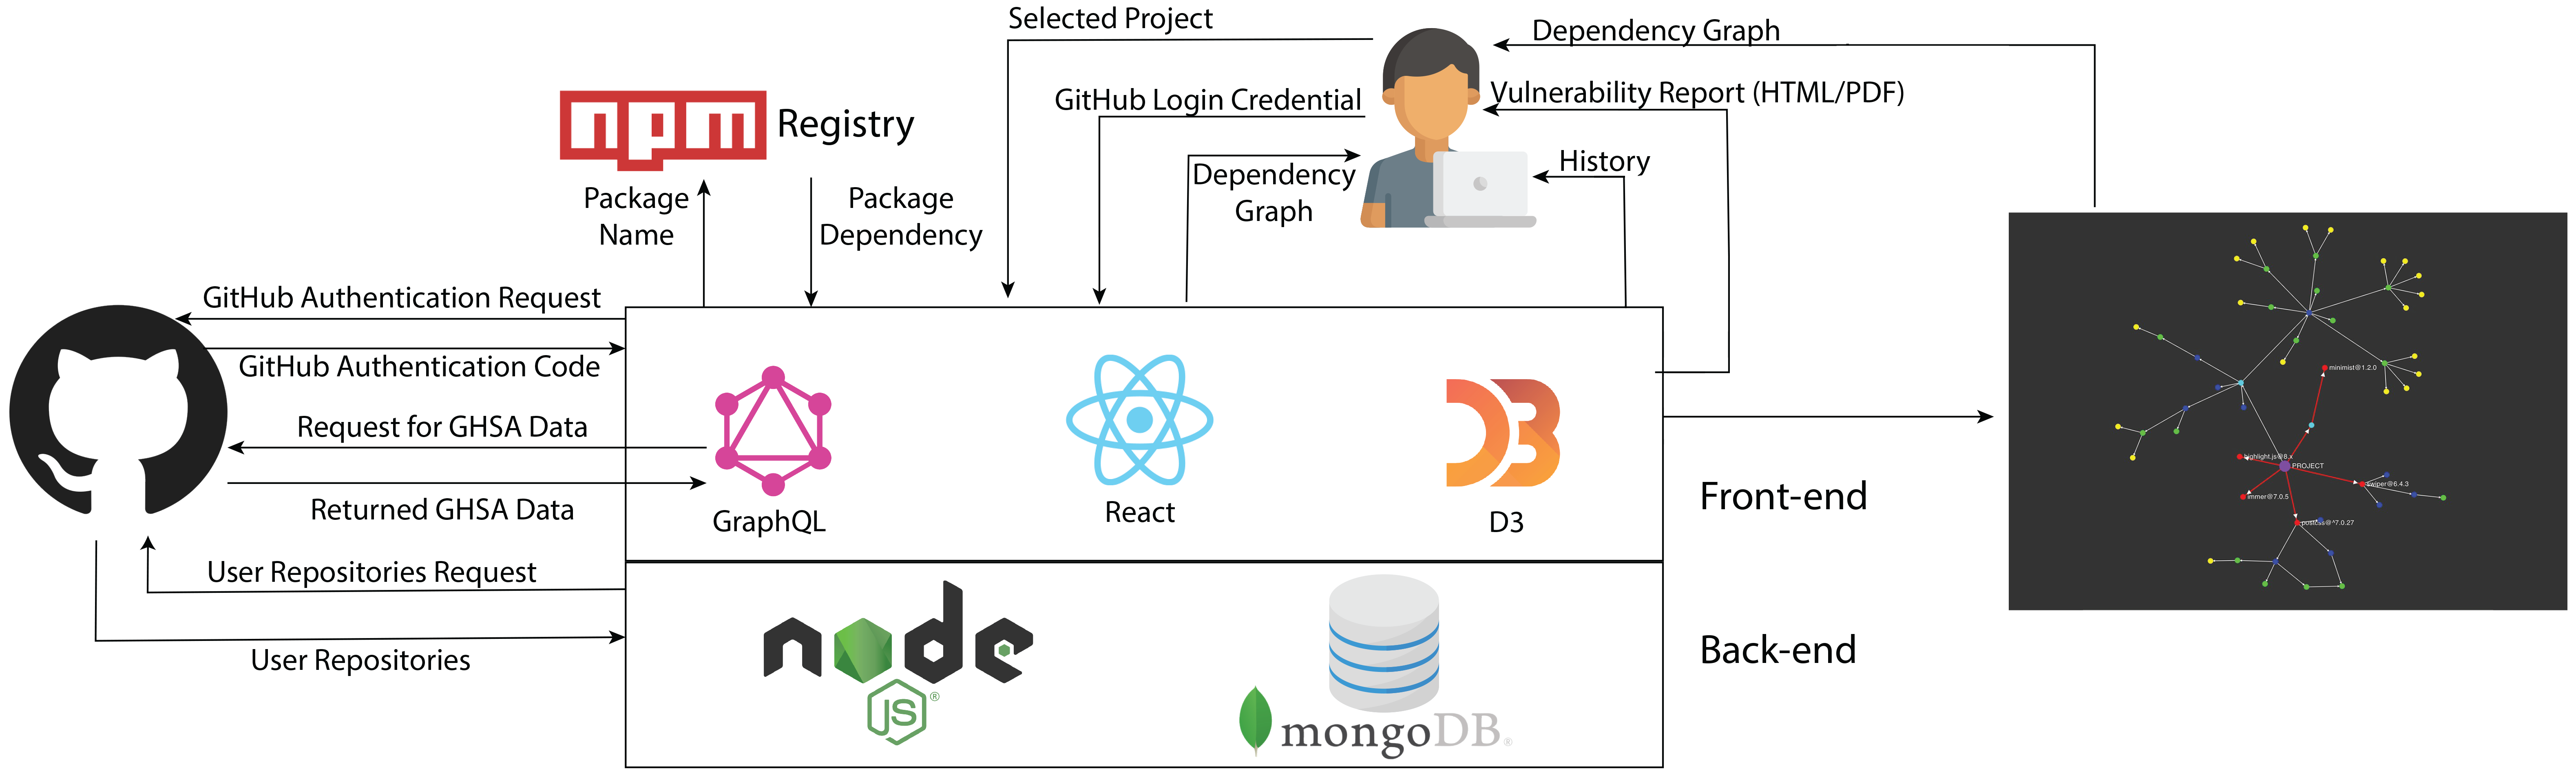
\includegraphics[width=2\columnwidth]{Figures/sys-arch-2.png}
		\caption{System Architecture of Achilles}
		\label{fig:system_architecture}
	\end{figure*}
	
	\subsection{Developer Struggles with Updating}
	Updating the dependencies is an essential task for software project.
	The new release of dependencies introduces new features and fixes to address bugs or security vulnerabilities.
    However, prior studies showed that developers are slow in updating their dependencies.
    The list of related studies is shown below.
% 	\citep{Robbes:2012, Hora:2015, Sawant2016, Bavota:2015, Ihara:2017}. \todo{Bodin please expand}
	\citet{Robbes:2012} and \citet{Sawant2016} studied how developers react to deprecated APIs.
	They found that only a minority of software projects upgrades their APIs and tends to use the older versions instead.
	\citet{Ihara:2017} showed that software projects do not always use the latest version of their dependencies.
	\citet{Decan:2017} investigated the evolution and issues of dependencies from different ecosystems.
	They revealed that these ecosystems have the issue of dependency updates.
	This issue not only affect the direct users of dependencies, but also the indirect users of such dependencies.
	\citet{Bogart:2015} conducted a survey and found that developers prefer to keep outdated dependencies as they afraid the new version might breaks their code.
% 	\citet{Decan:ICSME:2018} conducted an empirical study of technical lag in the npm ecosystem and found that the lags occur as the semantic versions of dependencies are not cover the latest release.
% 	They also found that using proper semantic versioning could reduces the technical lag.
	
	Security vulnerabilities from third-party dependencies is one of the issues that was raised to the attention of the open source software communities in recent years~\citep{Web:octoverse}.
	Their are several studies that investigate the impact of vulnerabilities within different ecosystems (e.g., npm, PyPI)~\citep{Kikas:2017, Linares:2017, Lauinger2016ThouSN, Decan:2018}.
	Their results share a similar view that a lot of dependencies were vulnerable regardless which ecosystem they belong to.
	The important updates such as vulnerability fixes and new major versions that introduce new features also influence how long developers would adopt these updates.
% 	\citet{Decan:2018} investigated the impact of vulnerabilities within the npm ecosystem.
	\citet{Decan:2018} found that the vulnerabilities are prevalent in the dependencies, while the developers of the vulnerable dependencies took several months to release the fixes.
	\citet{Chinthanet2021} focused on the lags of update in the case of vulnerability fix releases in npm ecosystem.
	They confirmed that despite the size of vulnerability fixes is small in terms of commit, developers still have a slow reaction to those fixes, which cause lags of updates throughout the dependency network.
	They also found that the severity of vulnerabilities is one of the factors that influences such lags of update.
	
	\subsection{Analyzing and Fixing Vulnerable Dependencies}
	Nowadays, there are automated tools that can help developers analyzing dependency security vulnerabilities in their software projects. Two tools that are widely used include GitHub Dependabot and npm audit. We explain each of them below.
	
	\subsubsection{GitHub Dependabot}
	Dependabot is a bot that analyzes a GitHub repository and automatically creates pull requests to update outdated and vulnerable dependencies. It is acquired by GitHub in 2019.
% 	In 2019, GitHub acquired Dependabot, the bot that automatically creates pull requests to keep dependencies in a GitHub repository secure and up-to-date.
	Dependabot currently supports repositories written in 15 programming languages.
	The process of Dependabot consists of three steps: (i) the bot finds outdated or vulnerable dependencies, (ii) the bot opens a pull request for each dependency, and (iii) the developers check the changes and merge them to the repository.
	% The recent work from Alfadel et. al. investigated the degree to which developers adopt the bot in their repositories \cite{Alfadel:MSR2021}.
	% They found that developers are highly receptive to pull requests from Dependabot.
	However, the limitation of Dependabot is that it only detects vulnerabilities in direct dependencies\footnote{\url{https://github.com/Dependabot/Dependabot-core/issues/2640}}.
	
	\subsubsection{npm audit}
	In 2018, npm introduced the new command for assessing the vulnerability from npm package dependencies called npm audit.
	The command submits the list of dependencies from \texttt{package.json} file (i.e., package metadata file) to the npm registry for a vulnerability report.
	Node.js developers could receive the vulnerability report while installing the dependencies from npm by default.
	Developers are also able to call an \texttt{npm audit} command manually when they need. npm audit can report software vulnerabilities in both direct and indirect dependencies. 
	However, the tool is only available as a command line tool with the vulnerability report in a tabular format.
	
% 	The two tools can support the developers by informing them of vulnerable dependencies. Nonetheless, they are both text-based and the developers need to figure out by themselves how the vulnerable dependencies connect to other dependencies. %Also, the developers need to investigate the vulnerabilities further by themselves according to the information of CVE given in the Dependabot or npm audit report.
	
	\section{Achilles}
	In this section, we present our prototype tool that is able to visualize the dependencies and their connections, and provide interactive information of security vulnerabilities, which has potential for a developer to prioritize their dependency updates. 
	
	\subsection{Technologies and Walk-through Design}
	
	As shown in Figure~\ref{fig:system_architecture}, we create a web-based prototype tool called ``\texttt{Achilles}\footnote{The name \texttt{Achilles} has been chosen as a metaphor of Achilles' heel, which represents a weakness in a software project.}'' for demonstrating the concept of dependency graph visualization. \texttt{Achilles} connects to GitHub and retrieves the user's npm repositories. It then analyzes the repository's dependencies and produces the dependency graph visualization and a security analysis report.  the tool consists of the front-end and the back-end parts. The front-end part consist of GraphQL, React, and D3.js libraries. The back-end parts consists of Node.js and MongoDB Atlas database.
	
	The \texttt{Achilles} tool analyzes security vulnerabilities in an npm project and creates a dependency graph visualization as follows.
	First, the React library handles the user interface and interactions with the users. After a user logs in with his or her GitHub account, Node.js is used to query the user's list of repositories. After the user selects a \texttt{package.json} file, which contains the list of npm dependencies, \texttt{Achilles} analyzes the relationships between the project and their packages using the data from the selected \texttt{package.json} file. This is when the tool gets all the direct dependencies. Then, \texttt{Achilles}  uses the list of the direct dependencies to send requests to the npm registry using GraphQL to retrieve the indirect dependencies. Currently, \texttt{Achilles} can retrieve dependency information up to 4 levels, i.e., the direct dependencies (level 1) and 3 levels of their indirect dependencies.
	After that, the collected dependency information is used to build a dependency graph using D3.js. The dependency graph visualizes the relationships between the project and its direct and indirect dependencies.
	
	Second, the automated analysis of dependency security vulnerability is performed by visiting each node in the graph and checking if the dependency in that node is vulnerable. The tool queries the vulnerability information from GitHub Advisory Database\footnote{\url{https://github.com/advisories}} using GraphQL. 
	
	Lastly, \texttt{Achilles} also makes use of the interactions of web interface provided by JavaScript and the D3.js library to display the dependency's vulnerability information as an interactive tool tip. The tool tip information is only displayed when a user hovers the cursor over a node in the graph.
	Thus \texttt{Achilles} only shows relevant security information that the user is interested in. 
	% If one of the nodes in the chain has found to be vulnerable, all the dependencies in that chain are marked as \textit{potentially vulnerable} by changing the node's color to red.
	% The edges connecting such nodes are also highlighted in red. Finally, the tool keeps the user's analysis history in MongoDB Atlas database.
	
	%In Achilles software system architecture (Figure \ref{fig:system_architecture}), we chose MongoDB Atlas database to store user and report information. We decided to choose this database because the data structure of the report that we need to store in database has various form of data such as vulnerable chaining node and vulnerability information that we get from GitHub Security Advisory which is returning JSON format. Moreover, MongoDB Atlas can store the data that is similar to the objects in the applications which benefits in reducing time in the need of translating the form of data that is stored in the database and the the form of data that is used in the code.
	
	%Users can interact with the Achilles software to see the visualization of the dependency graph via the website, which we developed using React, a front-end framework for developing a website, and D3.js library, which is used to create the visualization. Public GitHub repositories can be retrieved without any authorization. However, users are required to sign in with GitHub in order to allow our system to access their private repositories.
	
	%The Achilles software is developed using node.js to query data from MongoDB, get the users’ authentication from GitHub, retrieve users’ repositories information, and retrieve the package.json file.
	\begin{figure}
		\centering
		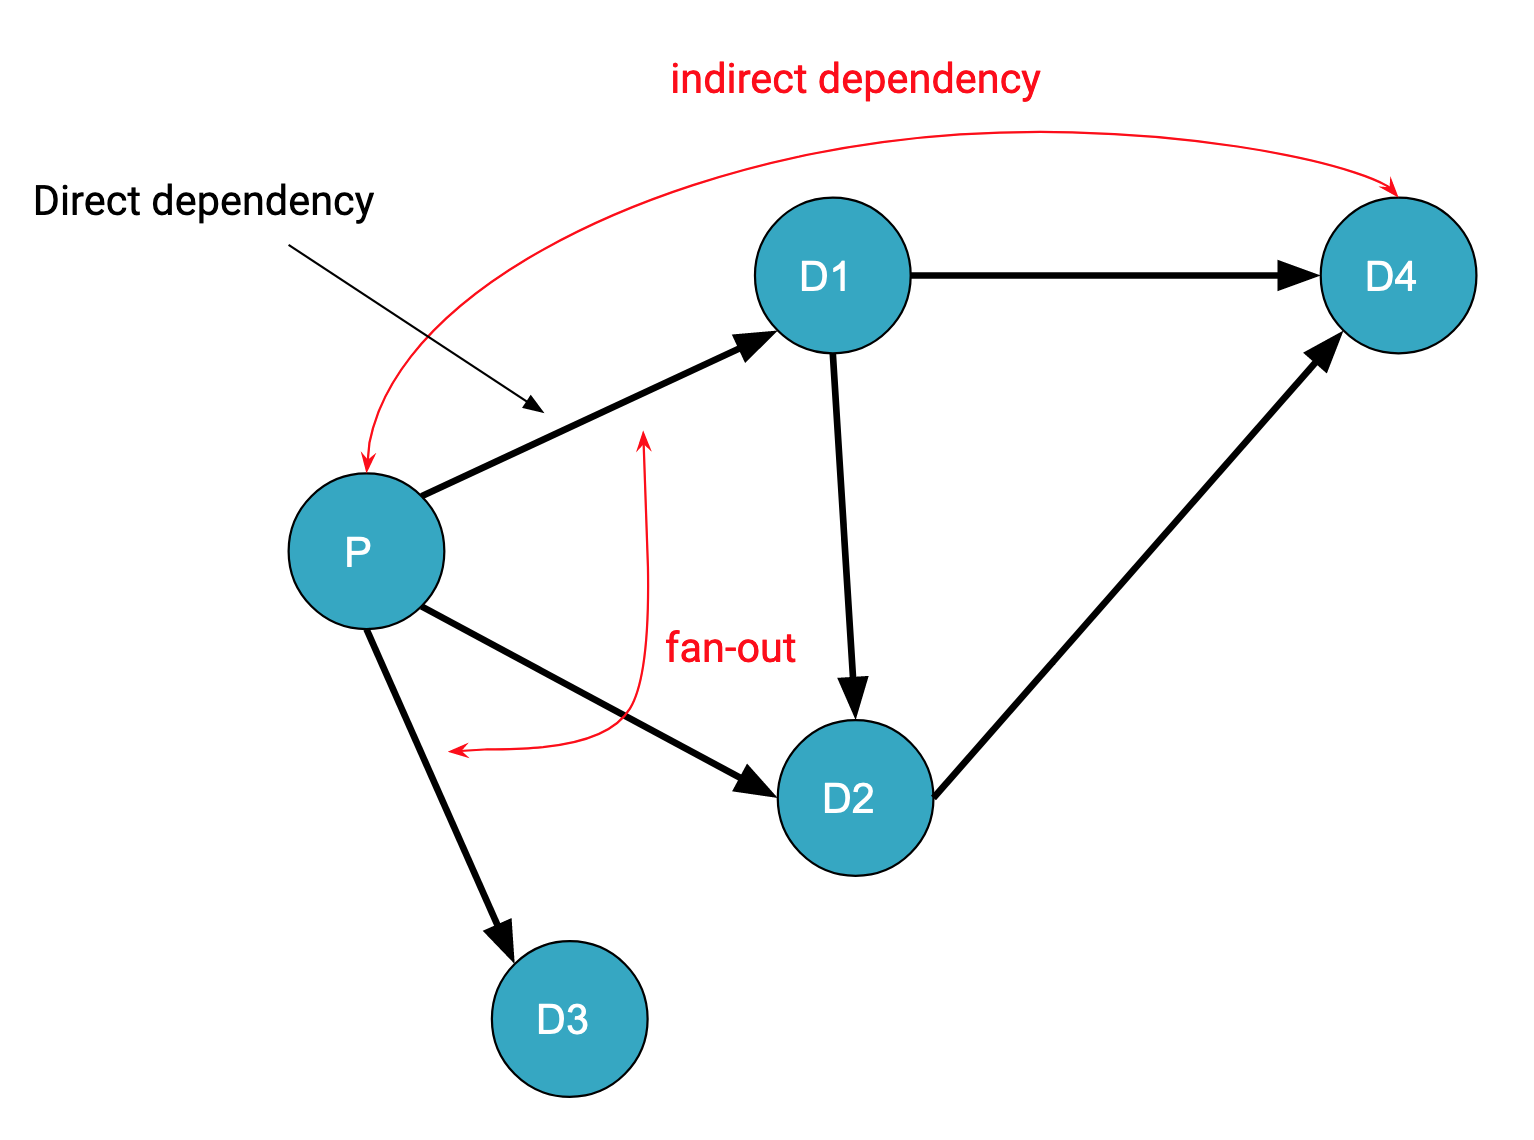
\includegraphics[width=0.9\linewidth]{Figures/Viz-concept-2}
		\caption{Using a dependency graph to depict direct and indirect dependencies.}
		\label{fig:viz-concept-2}
	\end{figure}
	
	\subsection{The Dependency Graph Visualization Design}
	According to the concept presented by Herman et al.~\cite{Herman2000}, we found that the npm dependencies and their relationships match well with graph visualization. In the graph visualization, the data can be represented by the nodes of a graph, with the edges representing their relations. We apply the graph visualization to represent dependencies in npm projects by using nodes to represent all the dependencies in the project and edges to represent how they depend on each other.
	
	Figure~\ref{fig:viz-concept-2} shows how we apply the graph visualization to npm dependencies. We have an npm project \texttt{P} which uses 3 dependencies, \texttt{D1}, \texttt{D2}, and \texttt{D3}. Their relationship can be captured in a directed graph as shown in the figure. Node \texttt{P} has an edge pointing to the node \texttt{D1}, \texttt{D2}, and \texttt{D3} showing that it depends on these three dependencies. Moreover, the dependency \texttt{D1} also depends on the existing dependency \texttt{D2}, and a new dependency \texttt{D4}. At the same time, \texttt{D2} also depends on \texttt{D4}. Thus, there are edges from the node \texttt{D1} to \texttt{D2} and to \texttt{D4} and another edge from the node \texttt{D2} to \texttt{D4}. 
	
	\subsubsection{Direct and Indirect Dependencies}
	%Since dependencies in npm projects have a relationship between each other, we defined the node to represent a dependency (i.e., package in npm) and the edge to represent the usage of one dependency on the other.  
	%The graph visualization can capture direct and indirect dependencies. 
	From the graph visualization in Figure~\ref{fig:viz-concept-2}, we can easily identify the direct and indirect dependencies. The nodes that have the path length of 1 from the project node \texttt{P} in the graph are direct dependencies (\texttt{D1}, \texttt{D2}, \texttt{D3}). The rest are indirect dependencies (\texttt{D4}). Furthermore, we can also see the fan-out of each node, i.e., how many dependencies such node have.  For example, in this figure, we can see that the project \texttt{P} has a fan-out value of 3 by having 3 outgoing edges to \texttt{D1}, \texttt{D2}, and \texttt{D3} respectively.
	
	
	
	\subsubsection{Choice of Colors}
	Figure~\ref{fig:viz-concept} shows how we represent the status of each dependency using colors. The project node is shown in \textcolor{purple}{purple} and is slightly bigger than other nodes.
	The vulnerable nodes are shown in \textcolor{red}{red} to make them easily distinguishable from the others. The normal nodes are shown in different colors.
	The direct dependencies are shown in \textcolor{lightblue}{cyan}. The indirect dependencies are shown in \textcolor{blue}{navy blue}, \textcolor{darkgreen}{green}, and \textcolor{darkyellow}{yellow} according to how many steps they are from the project node. This use of different colors for each type of nodes helps to easily locate the dependencies that are of the same or different type.
	
	In addition, \texttt{Achilles} also shows the edges in a chain of dependencies that contains a vulnerable node in \textcolor{red}{red}. So, all the dependencies in the vulnerable dependency chain can be easily located. On the other hand, normal chains of dependencies have black-color edges.
	
	\begin{figure}[tb]
		\centering
		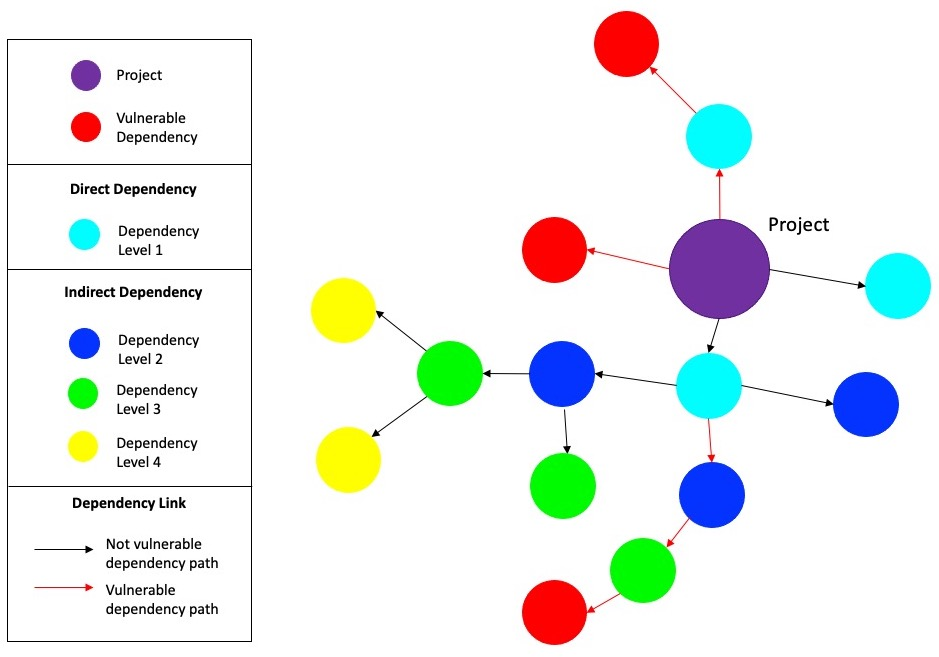
\includegraphics[width=\columnwidth]{Figures/Viz-concept-1.jpg}
		\caption{Meaning of node and edge colors in the dependency graph visualization}
		\label{fig:viz-concept}
	\end{figure}
	
	\begin{figure}
		\centering
		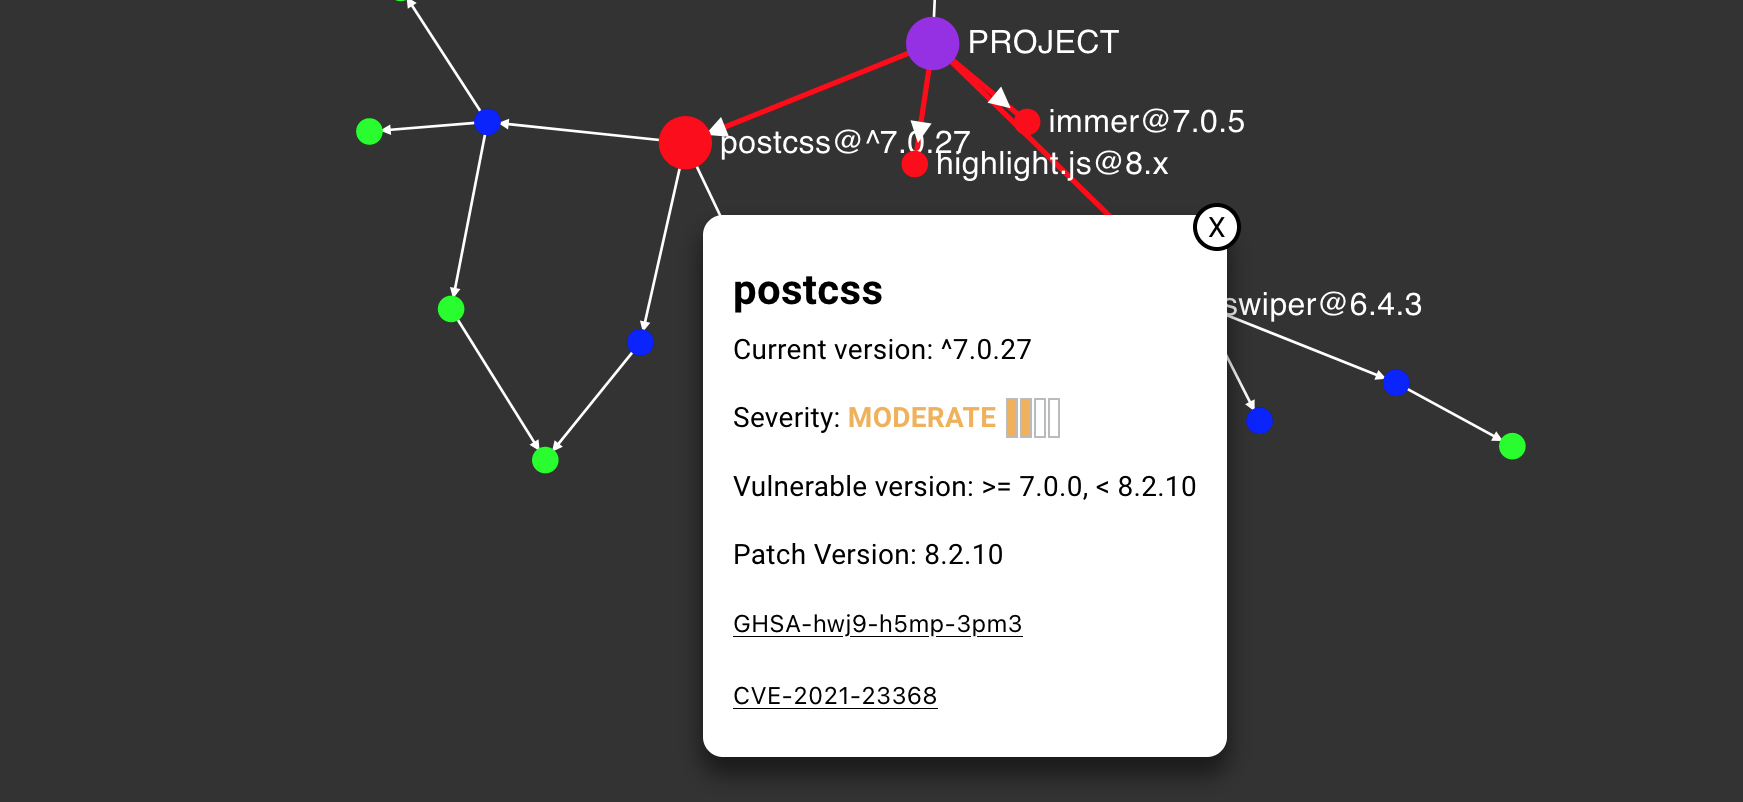
\includegraphics[width=\columnwidth]{Figures/tooltip_moderate}
		\caption{Vulnerable node: A tool tip that shows the dependency's vulnerability information}
		\label{fig:tooltip_moderate}
	\end{figure}
	
	\begin{figure}
		\centering
		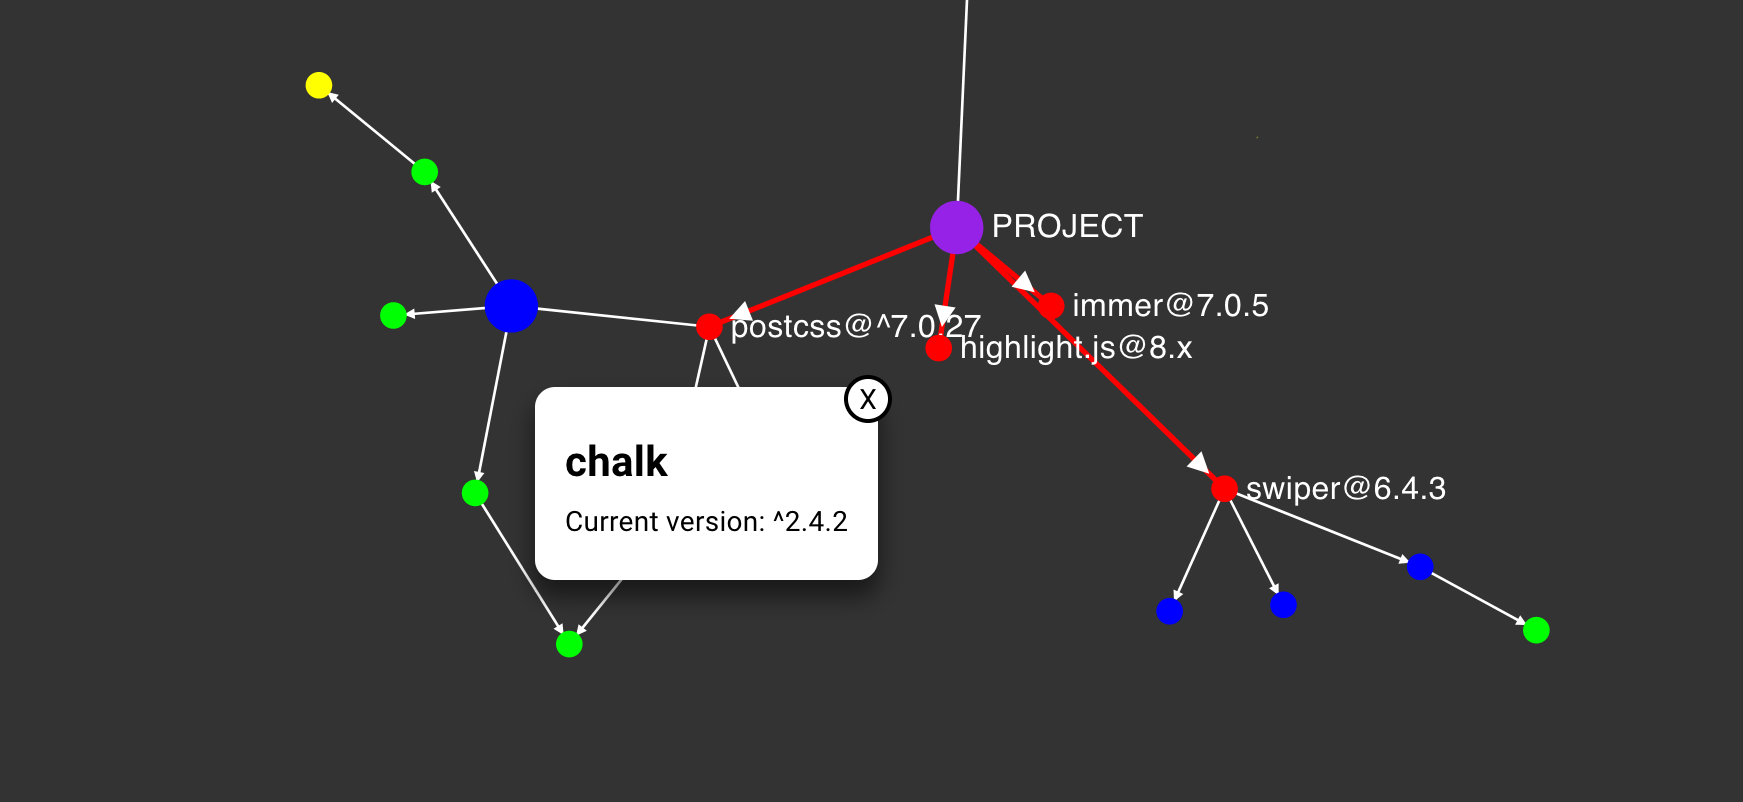
\includegraphics[width=\linewidth]{Figures/tooltip_normal}
		\caption{Normal node: A tool tip that shows the version of dependency}
		\label{fig:tooltip_normal}
	\end{figure}
	
	
	\begin{figure}[tb]
		\centering
		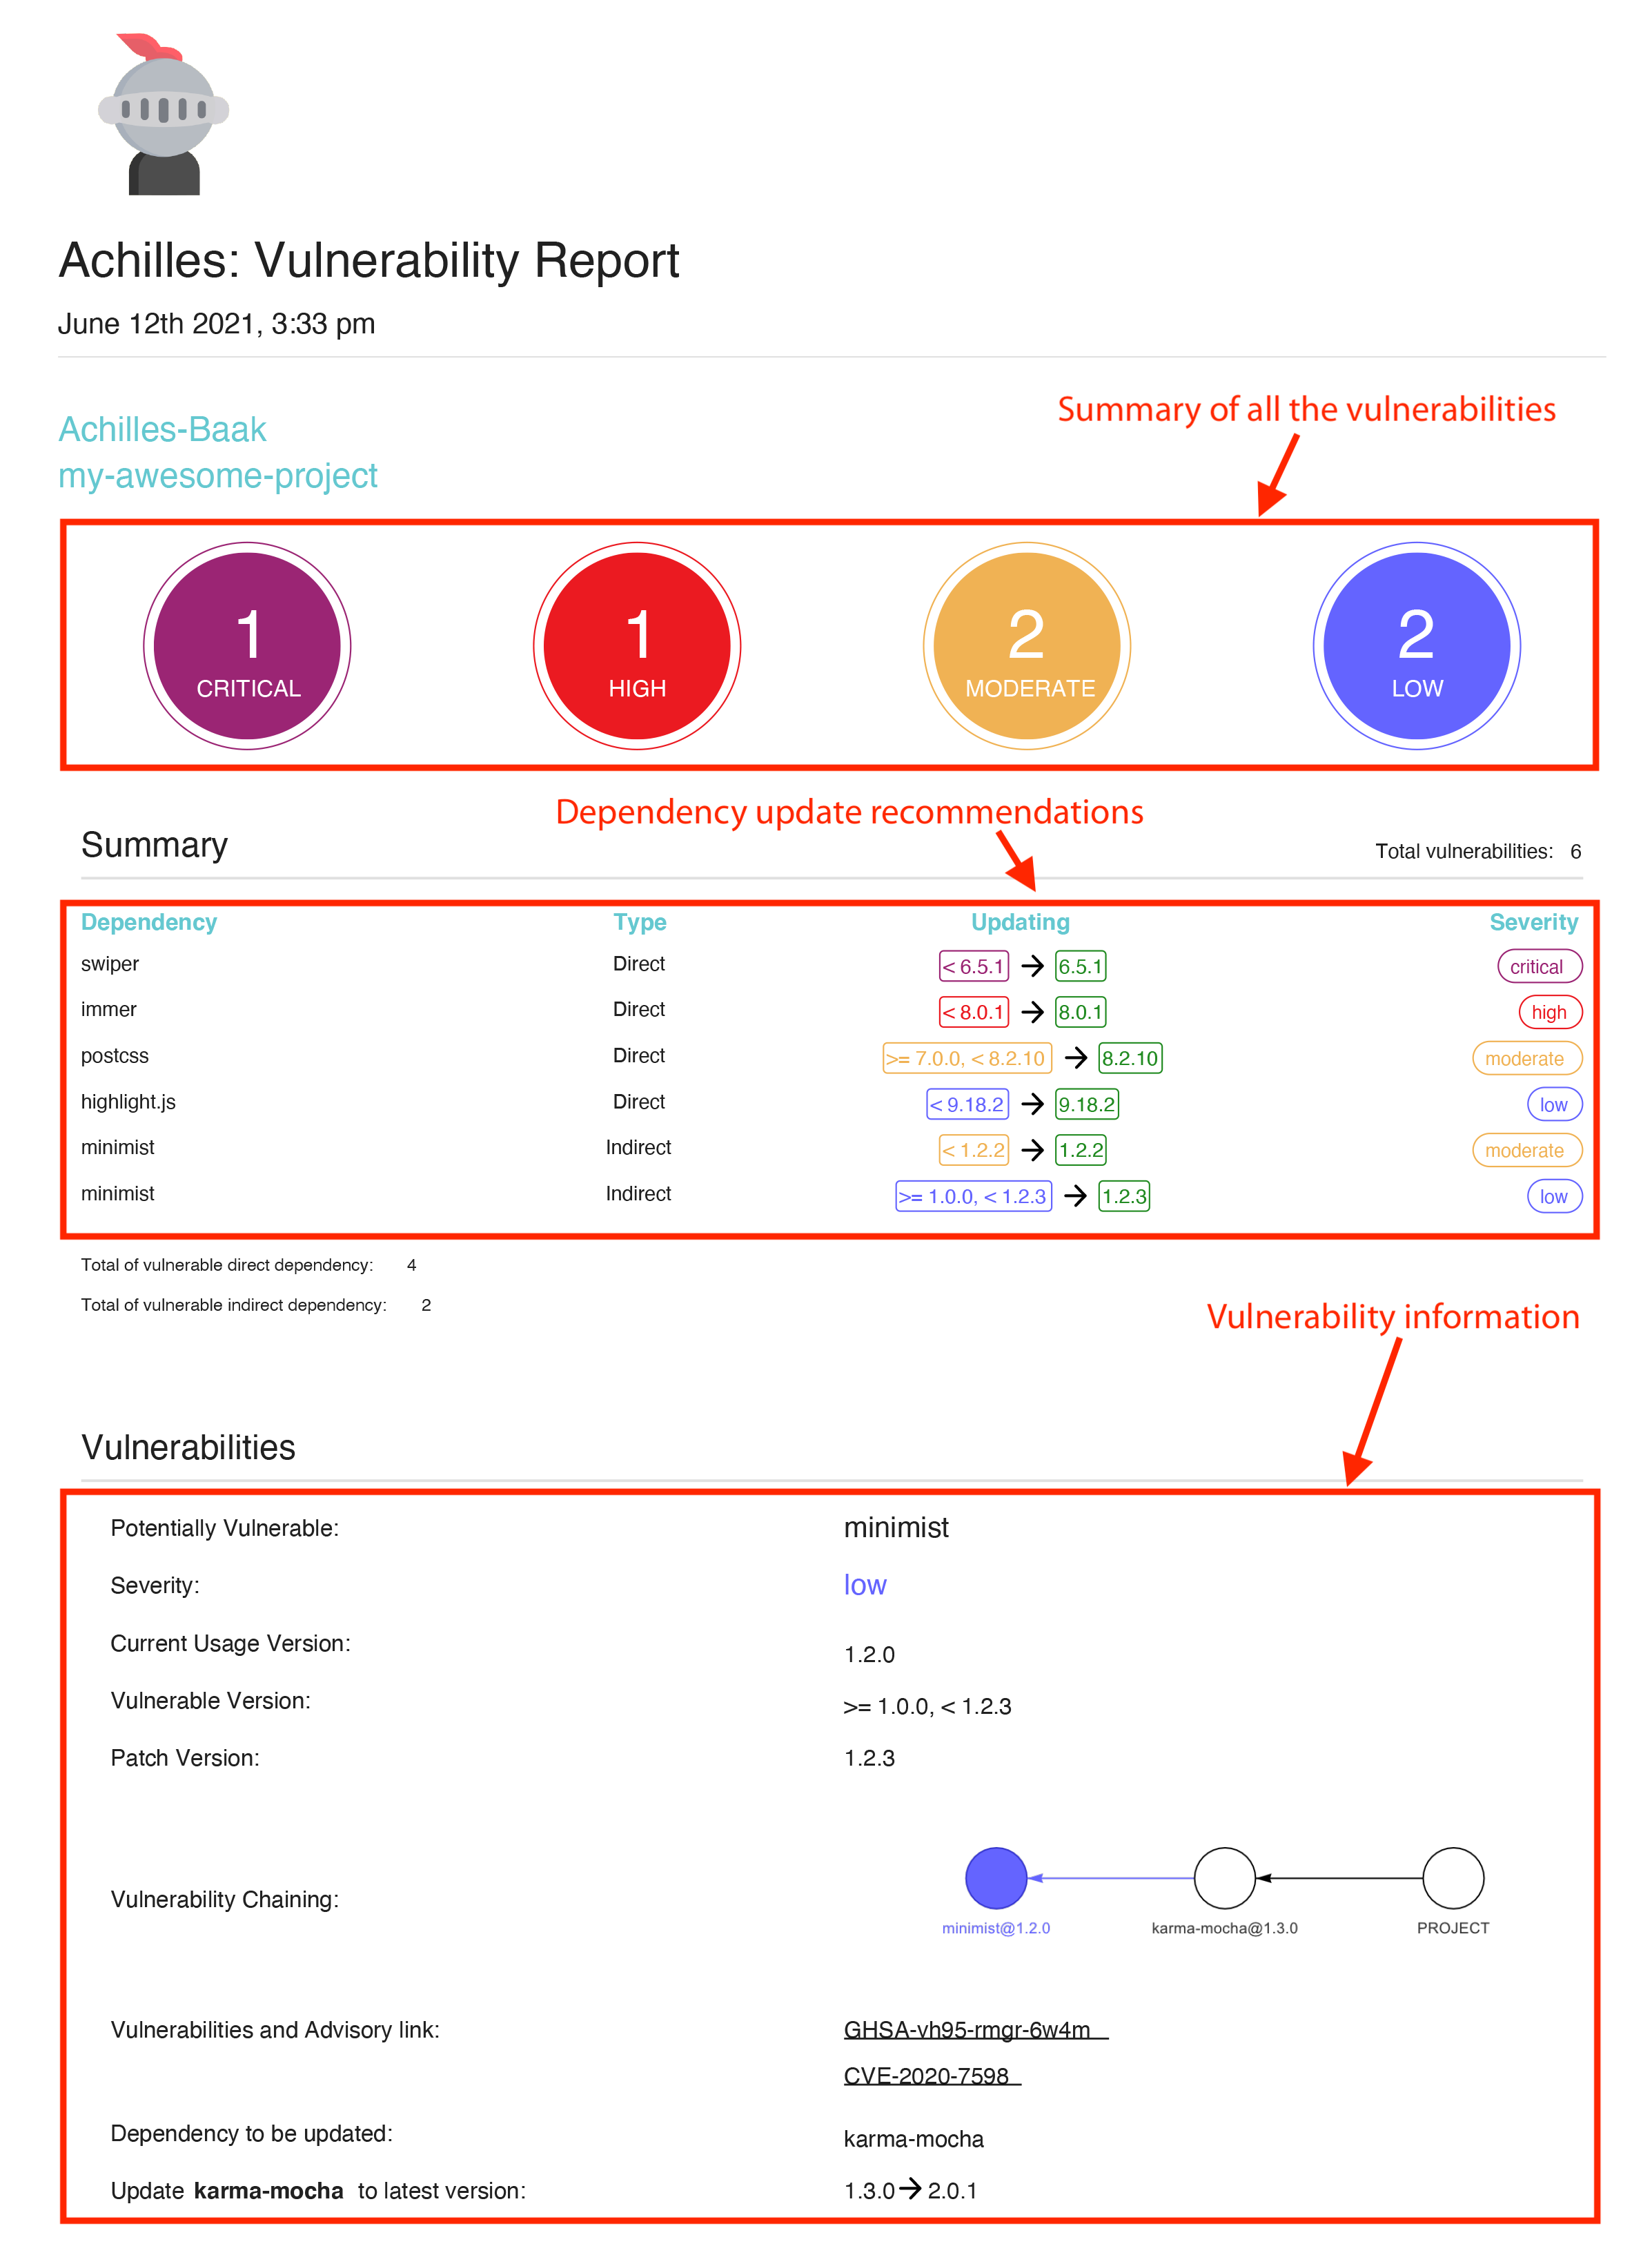
\includegraphics[width=\columnwidth]{Figures/my-awesome-project-achilles-report-1.png}
		\caption{\texttt{Achilles} vulnerability report}
		\label{fig:vul-report-1}
	\end{figure}
	
	\subsubsection{Tool Tip for Displaying Dependency's Vulnerability Information}
	Figure~\ref{fig:tooltip_moderate} and Figure~\ref{fig:tooltip_normal} show examples of the tool tip. If the hovered node is vulnerable, \texttt{Achilles} shows a tool tip with the vulnerability information including the dependency version, its vulnerability severity (low, medium, high, critical), the range of the versions that are affected by the vulnerability, the patch version of this vulnerability, and the links to the vulnerability's CVE.
	The user can use this information for their further investigation of the vulnerability and support their decision on making updates. For normal nodes, the tool tip shows the version of the dependency (as shown in Figure~\ref{fig:tooltip_normal}).
	
	\subsubsection{The Vulnerability Report}
	Figure~\ref{fig:vul-report-1} shows a vulnerability report that can be generated after an analysis of the dependency vulnerabilities is done. The report shows the summary of all the security vulnerabilities found in the analyzed npm project. On the top, the report contains the summary of all the vulnerabilities found categorized by their severity levels. 
	In the middle, it shows the recommendations of updating the vulnerabilities to their patch versions. Lastly, the remaining part of the report contains detailed information of each vulnerability, similar to the information displayed in the tool tip. 
	A graph showing the chain of dependencies of the vulnerability is also included along with the link to the corresponding GHSA entry, the CVE record, and the CWE records of such vulnerability. 
	The report can be saved for future references in PDF format.

	\section{Evaluation Setup}
	We performed a user study to evaluate the effectiveness of the dependency graph visualization provided by \texttt{Achilles}.
	The objective of the user study is to investigate how the dependency graph visualization supports developer’s decision on prioritizing vulnerabilities to fix and also to compare \texttt{Achilles} to Dependabot and npm audit. 
	
	\subsection{Research Questions}
	To guide our experiments, we ask the following two research questions in this study.
	
	\begin{itemize}
		\item \textbf{RQ1: How does using a dependency graph visualization support developer’s decision on prioritizing vulnerability to fix?} In this RQ, explore whether or not the visualization can influence a developer to re-prioritize their vulnerable dependency updates.
		\item \textbf{RQ2: How does using a dependency graph visualization perform compared to the state-of-the-art tools?} In this RQ, we compare against the other tools, to note any differences in the priority when updating a vulnerable dependency.
	\end{itemize}
	
	To answer our research questions, we conducted a user study by following the guidelines from \citet{Ko2013}.
% 	We highlight the key steps from the guidelines, which consists of Recruitment, Selection, Consent, Procedure, Demographic measurements, Group assignment, Training, Tasks, Outcome measurements, and Debrief and compensate. 
	
		\begin{table}[tb]
		\centering
		\caption{The participants' group assignment}
		\begin{tabular}{lrl}
			\toprule
			Group & Participants & Tools \\
			\midrule
			Experimental group & 10 & Dependabot $\rightarrow$ \texttt{Achilles} \\
			\midrule
			Controlled group & 10 & Dependabot $\rightarrow$ npm audit \\
			\bottomrule
		\end{tabular}
		\label{table:group_assignment}
	\end{table}
	
	\subsection{Experiment Protocol}
	We recruited twenty participants for the user study.
	Following the between-subject experimental design~\citep{Charness2012}, we randomly assign the participants into two groups: the controlled group and the experimental group, as shown in Table~\ref{table:group_assignment}. The controlled group has ten participants. The participants in this group used npm audit to analyze security vulnerabilities. For the experimental group, the ten participants used \texttt{Achilles} the perform the same tasks. 
	We used the control group as a baseline to compare our findings with those exposed to our tool and those that are not.
	
	\subsection{Recruitment and Selection}
	Table~\ref{table:participants} describes the demographics of the participants of the study.
	We set the inclusion criteria for selecting the participants of this experiment as follows:
	
	\begin{itemize}
		\item Participants must be computer science students or full-time employees at a software development company.
		\item Participants must have experience in programming for at least six months.
		\item Participants should understand and have fundamental knowledge in software vulnerabilities and related tools.
	\end{itemize}
	
	Then, we performed several methods to recruit the participants. For developers, we sent an email to invite them. For students, we directly contacted them.  Their demographics, their experience on using npm, and whether they know indirect dependencies along with their group assignments are shown in Table~\ref{table:participants}. Three participants were full-time developers. Six participants were master's students and eleven participants were undergraduate students. Six participants were proficient in using npm and six participants knew about indirect dependencies before the study.
	
	
	
	\begin{table}[tb]
		\caption{Participants’ Demographic}
		\centering
		\resizebox{0.5\textwidth}{!}{%
			\begin{tabular}{lllp{1.1cm}p{1.1cm}}
				\toprule
				Group & Participants & Demographics  & npm Exp. & Know Ind.~Dep? \\ 
				\midrule
				Experimental & E1                                          & Master's student & Low & No \\ 
				& E2                                          & Master's student & High & Yes \\ 
				& E3                                          & Undergrad student & High & Yes \\ 
				& E4                                          & Developer & Low & No \\ 
				& E5                                          & Undergrad student & High & Yes \\
				& E6                                          & Undergrad student & High & No \\
				& E7                                          & Undergrad student & Low & No \\ 
				& E8                                          & Master's student & Low & No \\
				& E9                                          & Master's student & Low & No \\
				& E10                                         & Master's student & Low & No \\
				\midrule
				Controlled & C1                         & Master's student & High & Yes \\ 
				& C2                                          & Undergrad student & Low & No  \\ 
				& C3                                          & Developer & High & Yes \\
				& C4                                          & Undergrad student & Low & No \\
				& C5                                          & Undergrad student & Low & No \\
				& C6                                          & Undergrad student & Low & Yes \\
				& C7                                          & Undergrad student & Low & No \\
				& C8                                          & Undergrad student & Low & No \\
				& C9                                          & Undergrad student & Low & No \\
				& C10                                         & Developer & Low & No \\
				\bottomrule
			\end{tabular}
		}
		\label{table:participants}
	\end{table}
	
	%When the actual experiment began, both group of participants were asked to see the security vulnerability report from Dependabot and prioritize the updates of the vulnerabilities. Then, for the controlled group, they were asked to use npm audit. On the other hand, the experimental group were asked to use Achilles to find security vulnerability. After that the participants in the two groups were asked to prioritize the updates of the vulnerabilities again. Finally, we interviewed the participants on their criteria that they use for their prioritization.
	
	%	\begin{figure}[tb]
	%		\centering
	%		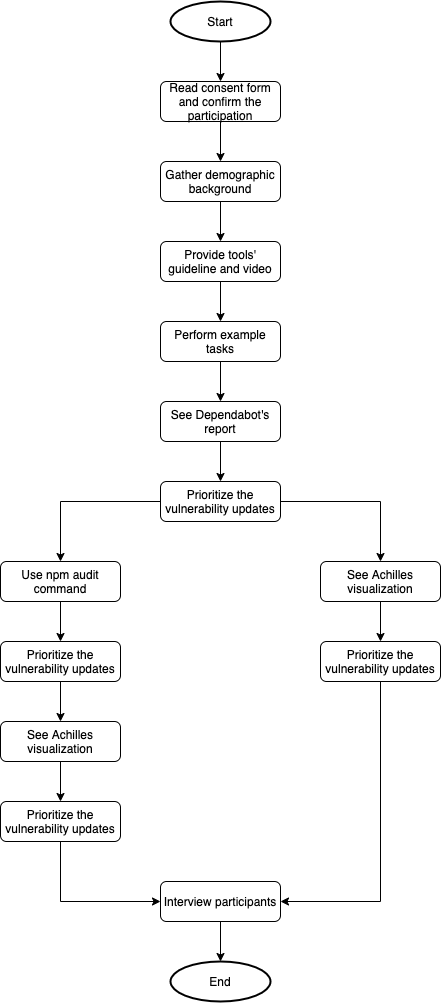
\includegraphics[scale=0.5]{Figures/fig1.png}
	%		\caption{Procedures of User Study}
	%		\label{fig:proceduresofuserstudy}
	%	\end{figure}
	
	
	%\subsubsection{Demographic measurements} - We asked participants the following questions prior the experiment in order to gain more understanding of participants' background.
	%\begin{itemize}
	%         \item How long have you been using npm?
	%         \item What do you use npm for?
	%         \item How often do you check security vulnerabilities in the project?
	%         \item Do you know indirect dependencies?
	%\end{itemize}
	
	%\subsubsection{Training} - We provided the tools guidelines and videos for the tools demonstration. We also prepare example tasks to check their understanding of the tools before we begin the experiments.
	

	
	\subsection{Experiment Tasks} 
	The participants were asked to perform two tasks of prioritizing vulnerable dependencies to fix in two npm projects. The participants needed to finish the first task before continuing to the second task. 
	\begin{itemize}
	    \item \textit{Task 1: Vulnerabilities with Complex Dependencies} We aim to test whether the dependency graph visualization would affect the participants’ decision on the dependency prioritization when the project contains complex dependencies. To achieve this, we created an npm project which contained four real-world vulnerable dependencies. 
	    
	     Figure \ref{fig:graphtest1} shows that visualization of the dependencies for Task 1.  From the visualization, we can see that the four selected dependencies are direct dependencies of the project. Furthermore, \texttt{pug} directly depends on eight other dependencies  and \texttt{type-graphql} directly depend on nine other dependencies (highlighted with blue nodes). Their dependencies also depend on several other dependencies (green and yellow nodes).
	
		Table~\ref{table:cha-teat1} shows the information of the dependencies in Task 1. 
	    We were interested in the dependencies which had different severity levels and also had different complexity levels. Thus, we selected two dependencies, \texttt{three} and \texttt{type-graphql}, that had high severity vulnerabilities and two dependencies, \texttt{xmldom} and \texttt{pug} that had low severity vulnerabilities. Two of the dependencies, \texttt{three} and \texttt{xmldom}, did not have any dependencies while the other two dependencies, \texttt{type-graphql} and \texttt{pug}, depended on a large number of dependencies, i.e., they introduced complexity into the chain of dependencies. 
	    We crossed check to make sure that the four selected vulnerable dependencies were reported by Dependabot, npm audit, and \texttt{Achilles}. We put them into 4 categories: HS (high-severity simple), HC (high-severity complex), LS (low-severity simple), and LC (low-severity complex).
	
	    \item \textit{Task 2: Vulnerabilities with Indirect Dependencies}
	    For Task 2, we aim to test whether the dependency graph visualization which shows the types of the vulnerabilities (direct or indirect) would affect the participants’ decision on dependency prioritization. We created another npm project for this task and also made sure they could be detected by the three tools. The selected four dependencies include \texttt{netmask}, \texttt{base64-url}, \texttt{angular-expressions}, and \texttt{minimist}. Two dependencies, \texttt{netmask} and \texttt{base64-url}, had high severity vulnerabilities, while \texttt{angular-expressions} and \texttt{minimist} had low severity vulnerabilities. 
	    
	    Figure \ref{fig:graphtest2} and Table \ref{table:cha-test2}  shows the information of the dependencies in Task 2 and how they depend on each other. We can see from the visualization that \texttt{angular-expressions} and \texttt{netmask} are the direct dependency of the project, while \texttt{minimist} and \texttt{base64-url} are indirect dependencies of the project.
	    Similarly to Task 1, we put them into 4 categories: HD (high-severity direct dependency), HI (high-severity indirect dependency), LD (low-severity direct dependency, and LI (low-severity indirect dependency).
	\end{itemize}

\begin{figure}[tb]
	\centering
	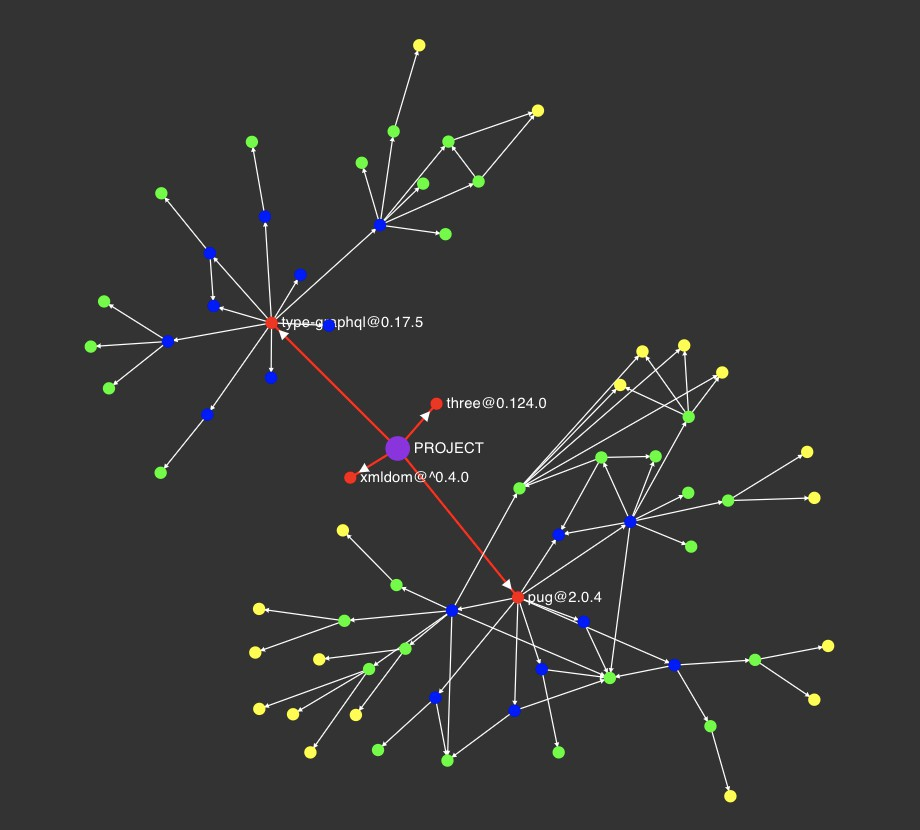
\includegraphics[width=0.9\columnwidth]{Figures/Achilles-Test1.jpeg}
	\caption{Dependency graph visualization of Task 1}
	\label{fig:graphtest1}
\end{figure}

\begin{table}[tb]
	\centering
	\caption{Task 1: Vulnerabilities with Complex Dependencies}
	\begin{tabular}{llcccc}
		\toprule
		No & Dependency & Version & Severity & Type & Category \\
		\midrule
		1 & three & 0.12.40 & High & Simple & HS \\
		2 & pug & 2.0.4 & High & Complex &  HC \\
		3 & xmldom & \^{}0.4.0 & Low & Simple & LS \\
		4 & type-graphql & 0.17.5 & Low & Complex & LC \\
		\bottomrule
	\end{tabular}
	\label{table:cha-teat1}
\end{table}

\begin{figure}[tb]
	\centering
	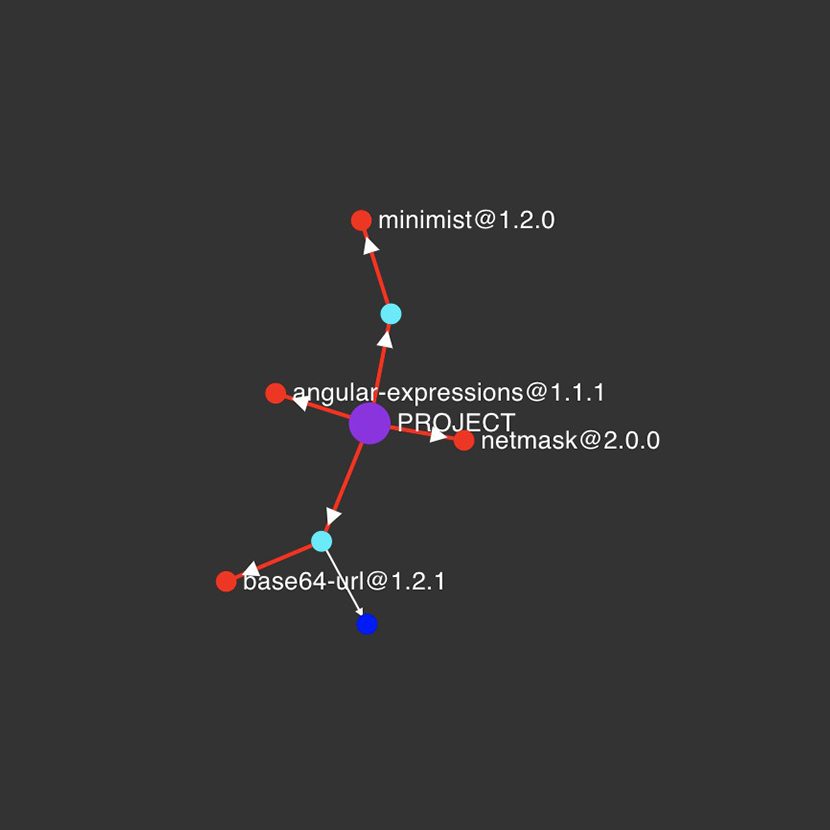
\includegraphics[width=0.8\columnwidth]{Figures/Achilles-Test2.png}
	\caption{Dependency graph visualization of Task 2}
	\label{fig:graphtest2}
\end{figure}
	
\begin{table}[t]
	\centering
	\caption{Task 2: Vulnerabilities with Indirect Dependencies}
	\begin{tabular}{llcccc}
		\toprule
		No & Dependency & Version & Severity & Type & Category \\
		\midrule
		1 & netmask & 2.0.0 & High & Direct & HD \\ 
		2 & base64-url & 1.2.1 & High & Indirect & HI \\
		3 & angular-expressions & 1.1.1 & Low & Direct & LD \\ 
		4 & minimist & 1.2.0 & Low & Indirect & LI \\
		\bottomrule
	\end{tabular}
	\label{table:cha-test2}
\end{table}

	\subsection{Experiment Procedure}
	
	For our experiment procedure, we started by letting the participants read the consent form and ask for their confirmation to join the experiment. Then, we gathered their demographic background, provided the guidelines and videos of the tools demonstration, and asked them to perform two example tasks to train them to get used to the tools and security vulnerabilities in npm projects.
	
	For each task, the participants had to do the following. Participants in both the controlled and the experimental groups were given an npm project and the vulnerability report of Dependabot (shown in Figure~\ref{fig:screenshot-dependabot}). Then, they were asked to rank the vulnerable dependencies that they thought they would fix from the first to the last. After that, a different tool was introduced to each group. For the controlled group, npm audit and its report was introduced (shown in Figure~\ref{fig:screenshot-npm-audit}). For the experimental group, \texttt{Achilles} and the dependency graph visualization was introduced (shown in Figure~\ref{fig:screenshot-achilles}). After using the given tool to explore the security vulnerabilities, the participants were asked to rank the vulnerable dependencies to fix again.
	
    Finally, we expose the control group to  \texttt{Achilles} after they had finished using npm audit. Then, they performed the dependency prioritization for the last time.

	\begin{figure*}
		\centering
		\begin{subfigure}[b]{0.32\textwidth}
			\centering
			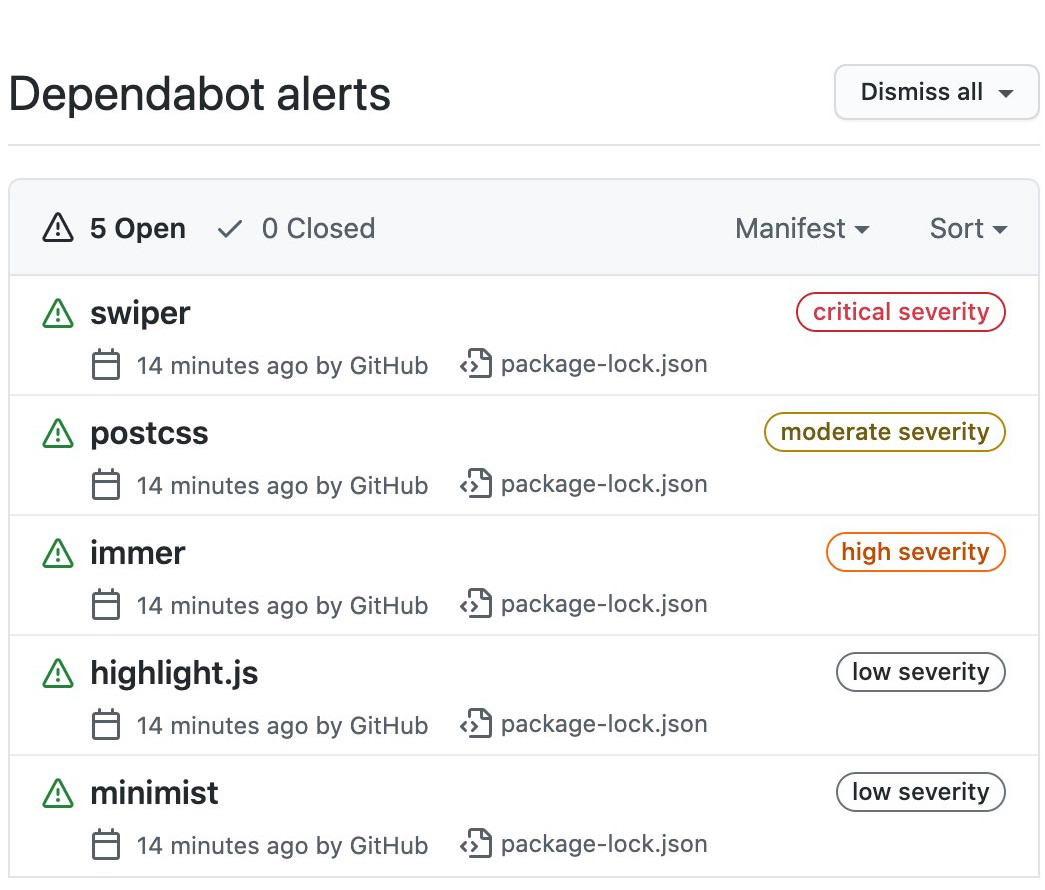
\includegraphics[width=\textwidth]{Figures/screenshot-dependabot.png}
			\caption{Dependabot}
			\label{fig:screenshot-dependabot}
		\end{subfigure}
		\hfill
		\begin{subfigure}[b]{0.32\textwidth}
			\centering
			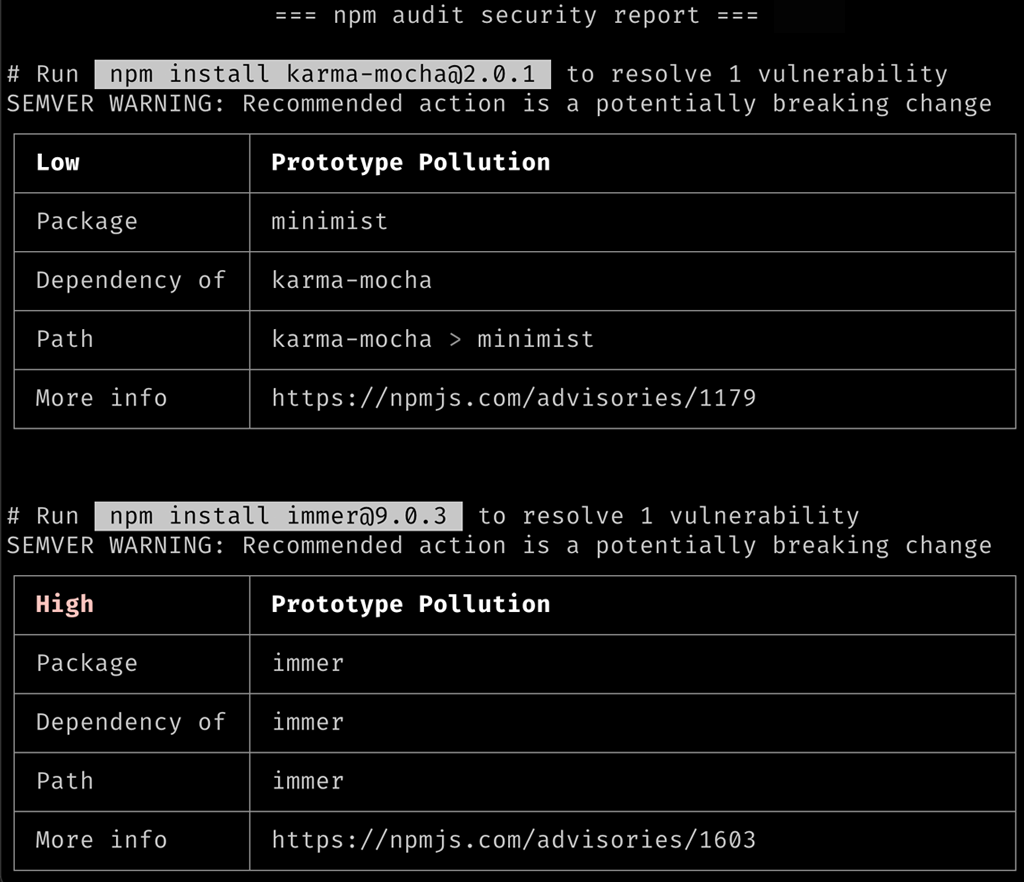
\includegraphics[width=\textwidth]{Figures/screenshot-npm-audit2.png}
			\caption{npm audit}
			\label{fig:screenshot-npm-audit}
		\end{subfigure}
		\hfill
		\begin{subfigure}[b]{0.32\textwidth}
			\centering
			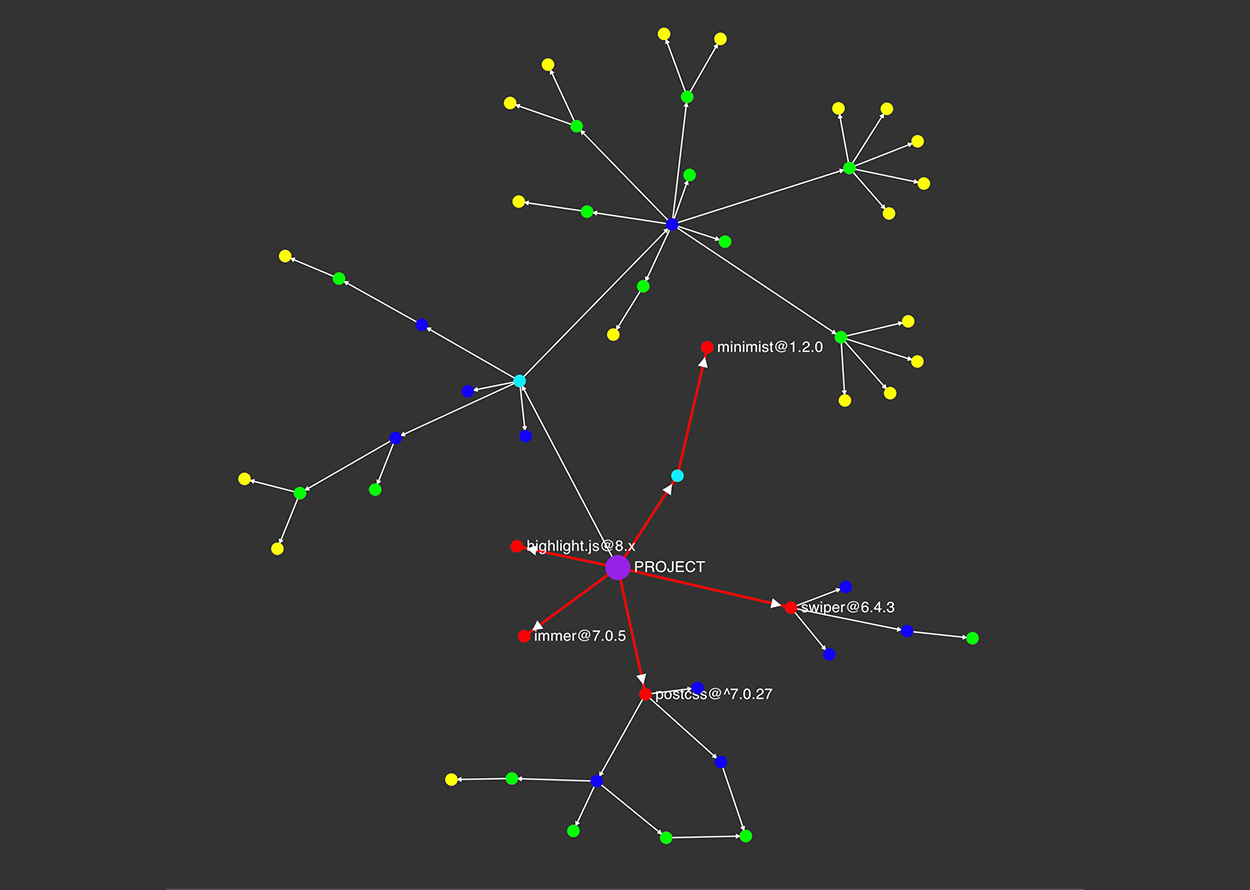
\includegraphics[width=\textwidth]{Figures/screenshot-achilles.png}
			\caption{Achilles}
			\label{fig:screenshot-achilles}
		\end{subfigure}
		\caption{The security reports of the three tools used in the user study}
		\label{fig:screenshots}
	\end{figure*}
		
	\subsection{Outcome measurements and analysis}

To answer RQ1, we would like to compare the differences between groups that change their priorities after begin exposed to the different tools. 
 We call them the \textit{re-prioritize group} and the \textit{unchanged priority group}. 
 The re-prioritize group contains the participants whose the dependency prioritization after seeing \texttt{Achilles} report differ from the  initial prioritization based on Dependabot report, i.e., they changed their ranking of the vulnerable dependencies to be fixed. 
 The unchanged priority group contains the participants who the dependency prioritization were the same between \texttt{Achilles} and Dependabot.
 
 To answer RQ2, we compared the prioritization results that the participants used before (i.e., based on the security vulnerability report from Dependabot) and after (i.e., based on the security vulnerability report from npm audit or \texttt{Achilles}) of the two tasks. 
 This is classified as being the same or different.
 We also record whether or not the priorities are the same or different when the controlled group finally gets exposed to \texttt{Achilles}.
 %We also compared the results between different types of visualization which are table by npm audit and graph by Achilles.
	
	%\subsubsection{Debrief} - We told the participants about the purpose of this experiment and interview them for them about the criteria that they used and the tool feedback.
	
	% \section{Participants’ demographic data
% 	\todo{stop here -Raula}
	\section{Results and Discussion}
	This section describes the results and discusses key observations from the user study.
	
	\subsection{Answering RQ1}
	
% 	\subsection{Task 1: Vulnerabilities with Complex Dependencies}
	
% 	\subsubsection{Experimental Group (\texttt{Achilles})}
	As shown in Table~\ref{table:result-Ach-t1}, for the experimental group for Task 1, the re-prioritize group includes 7 participants (E1, E2, E4, E5, E7, E8, and E9). We observed that they only emphasized on severity when they saw the vulnerability report from Dependabot. However, after they used \texttt{Achilles}, they also took other factors into account. 
	According to Table \ref{table:prioritization_factor} (Task 1), after seeing the vulnerability report from Dependabot, seven participants used severity as the significant factor for the prioritization. After using the dependency graph visualization in \texttt{Achilles}, there were six cases (E1, E2, E4, E5, E7, and E8) where the package complexity had become one of the factors when prioritizing the package update, either as the first or the second priority factor.
	On the other hand, the unchanged priority group (E3, E6, and E10) did not change their prioritization order. Nonetheless, they all mentioned that after they see \texttt{Achilles}, they realized the information about the package's complexity easier.
	
	\begin{table*}
		\caption{Task 1 Vulnerabilities with Complexities: Result by Participants}
		\centering
		\begin{tabular}{clll|clll}
			\toprule
			\multicolumn{4}{c|}{Experimental Group} & \multicolumn{4}{c}{Controlled Group}  \\ 
			\midrule
			Participants         & Tool       & Dependency Prioritization & Comparison & Participants & Tool  & Dependency Prioritization & Comparison \\ 
			\midrule
			\multirow{2}{*}{E1}   & Dependabot    & HC \textgreater{}= HS \textgreater LC \textgreater{}= LS & \multirow{2}{*}{Different} & \multirow{2}{*}{C1} & Dependabot & HS \textgreater HC \textgreater LS \textgreater LC & \multirow{2}{*}{Same} \\ 
			& \texttt{Achilles}      & HC \textgreater HS \textgreater LC \textgreater LS       & & & npm audit & HS \textgreater HC \textgreater LS \textgreater LC & \\ \midrule
			\multirow{2}{*}{E2}   & Dependabot    & HS \textgreater{}= HC \textgreater LC \textgreater LS    & \multirow{2}{*}{Different} & \multirow{2}{*}{C2} & Dependabot & HC \textgreater HS \textgreater LC \textgreater LS & \multirow{2}{*}{Different} \\ 
			& \texttt{Achilles}      & HC \textgreater LC \textgreater HS \textgreater LS       & & & npm audit & HC \textgreater HS \textgreater LC \textgreater{}= LS & \\ \midrule
			\multirow{2}{*}{E3}   & Dependabot    & HS \textgreater{}= HC \textgreater LC \textgreater{}= LS & \multirow{2}{*}{Same} & \multirow{2}{*}{C3} & Dependabot & HC \textgreater HS \textgreater LC \textgreater{}= LS & \multirow{2}{*}{Same} \\ 
			& \texttt{Achilles}      & HS \textgreater{}= HC \textgreater LC \textgreater{}= LS & & & npm audit & HC \textgreater HS \textgreater LC \textgreater{}= LS & \\ \midrule
			\multirow{2}{*}{E4}   & Dependabot    & HS \textgreater{}= HC \textgreater LC \textgreater{}= LS & \multirow{2}{*}{Different} & \multirow{2}{*}{C4} & Dependabot & HS \textgreater HC \textgreater LC \textgreater{}= LS  & \multirow{2}{*}{Different} \\ 
			& \texttt{Achilles}      & HC \textgreater HS \textgreater LC \textgreater LS       & & & npm audit & HC \textgreater HS \textgreater LS \textgreater LC & \\ \midrule
			\multirow{2}{*}{E5}   & Dependabot    & HC \textgreater HS \textgreater LS \textgreater LC       & \multirow{2}{*}{Different} & \multirow{2}{*}{C5} & Dependabot & HS \textgreater HC \textgreater LC \textgreater LS & \multirow{2}{*}{Same} \\ 
			& \texttt{Achilles}      & HS \textgreater HC \textgreater LS \textgreater LC       & & & npm audit & HS \textgreater HC \textgreater LC \textgreater LS & \\ \midrule
			\multirow{2}{*}{E6}   & Dependabot    & HC \textgreater{}= HS \textgreater LC \textgreater{}= LS & \multirow{2}{*}{Same} & \multirow{2}{*}{C6} & Dependabot & HS \textgreater{}= HC \textgreater LS \textgreater{}= LC & \multirow{2}{*}{Same} \\ 
			& \texttt{Achilles}      & HC \textgreater{}= HS \textgreater LC \textgreater{}= LS & & & npm audit & HS \textgreater{}= HC \textgreater LS \textgreater{}= LC & \\ \midrule
			\multirow{2}{*}{E7}   & Dependabot    & LS \textgreater LC \textgreater HS \textgreater HC       & \multirow{2}{*}{Different} & \multirow{2}{*}{C7} & Dependabot & LC \textgreater HS \textgreater LS \textgreater HC& \multirow{2}{*}{Same} \\ 
			& \texttt{Achilles}      & HS \textgreater{}= LS \textgreater HC \textgreater LC    & & & npm audit & LC \textgreater HS \textgreater LS \textgreater HC& \\ \midrule
			\multirow{2}{*}{E8}   & Dependabot    & HS \textgreater HC \textgreater LC \textgreater LS       & \multirow{2}{*}{Different} & \multirow{2}{*}{C8}  & Dependabot & HC \textgreater HS \textgreater LS \textgreater LC & \multirow{2}{*}{Different} \\ 
			& \texttt{Achilles}      & HS \textgreater{}= LS \textgreater HC \textgreater LC    & & & npm audit & HS \textgreater HC \textgreater LC \textgreater{}= LS & \\ \midrule
			\multirow{2}{*}{E9}   & Dependabot    & HS \textgreater LC \textgreater LS \textgreater HC       & \multirow{2}{*}{Different} & \multirow{2}{*}{C9} & Dependabot & HS \textgreater{}= HC \textgreater{}= LC \textgreater LS  & \multirow{2}{*}{Different} \\ 
			& \texttt{Achilles}      & HS \textgreater HC \textgreater LC \textgreater LS       & & & npm audit & HS \textgreater{}= HC \textgreater{}= LC \textgreater{}= LS & \\ \midrule
			\multirow{2}{*}{E10}  & Dependabot    & HC \textgreater{}= HS \textgreater LC \textgreater{}= LS & \multirow{2}{*}{Same} & \multirow{2}{*}{C10} & Dependabot & HC \textgreater{}= HS \textgreater LC \textgreater{}= LS & \multirow{2}{*}{Same} \\ 
			& \texttt{Achilles}      & HS \textgreater{}= HC \textgreater LC \textgreater{}= LS & & & npm audit & HC \textgreater{}= HS \textgreater LC \textgreater{}= LS & \\ \midrule
			\multicolumn{8}{l}{H = High severity, L = Low severity, C = Complex (has several dependencies), S = Simple (no dependency)} \\
		\end{tabular}
		\label{table:result-Ach-t1}
	\end{table*}
	
	\begin{table}[tb]
		\caption{Factors for Prioritizing Dependency Fixes in the Experimental Group}
		\centering
		\resizebox{0.49\textwidth}{!}{%
			\begin{tabular}{cp{2cm}p{2cm}p{1.5cm}r} 
				\toprule
				Tool & First factor & Second factor & Participants & Amount \\ 
				\midrule
				\multicolumn{5}{l}{\textit{Task 1 Complexity}}  \\
				\midrule
				\multirow{7}{*}{Dependabot} & High Severity & Low Severity & E1, E2, E3, E4, E5, E6, E10  & 7  \\ 
				& High Severity & Recent use  & E8 & 1 \\ 
				& Version No. & - & E9 & 1 \\ 
				& Indirect dep. & - & E7 & 1  \\ 
				\midrule
				\multirow{6}{*}{\texttt{Achilles}}  & High Severity & Low Severity                    & E3, E6, E10                                                            & 3               \\ 
				&  High Severity & High Complexity                 & E1, E4, E5                                                             & 3               \\ 
				&  High Severity & Low Complexity                  & E7                                                                     & 1               \\ 
				&  High Severity  & Version                         & E9                                                                     & 1               \\ 
				& High Complexity                         & High Severity                   & E2                                                                     & 1               \\ 
				& Low Complexity                          & High Severity                   & E8                                                                     & 1               \\ 
				\midrule
				\multicolumn{5}{l}{\textit{Task 2 Direct/Indirect Dependency}}  \\
				\midrule
				\multirow{7}{*}{Dependabot} & High Severity  & Low Severity                    & E1, E2, E4, E10                                & 4               \\ 
				& High Severity & Direct dep.                         & E5                                            & 1               \\ 
				& High Severity & Issue type                      & E6                                            & 1               \\ 
				& High Severity & Recent use                      & E8                                            & 1               \\ 
				& Direct dep.  & High Severity                   & E3                                            & 1               \\ 
				& Indirect dep. & Severity                        & E9                                            & 1               \\ 
				& Indirect dep. & - & E7                                            & 1               \\ 
				\midrule
				\multirow{5}{*}{\texttt{Achilles}}  & High Severity & Direct dep.                          & E1, E5, E6, E8, E10                           & 5               \\ 
				& Direct dep.  & High Severity                   & E2, E3, E4 & 3               \\ 
				& High Severity & Version                         & E9                                            & 1               \\ 
				& Indirect dep. & Severity                        & E7                                            & 1               \\ 
				\bottomrule
			\end{tabular}
		}
		\label{table:prioritization_factor}
	\end{table}
	
\begin{table}[tb]
		\centering
		\caption{Developers' Decisions Using \texttt{Achilles} and npm audit Compared to Dependabot}
		\begin{tabular}{llrr}
			\toprule
			Task & Decision & \texttt{Achilles} & npm audit \\
			\midrule
			\multirow{2}{*}{Task 1} & Same & 3 & 6 \\ 
			& Different & 7 & 4 \\ \midrule
			\multirow{2}{*}{Task 2} & Same & 3 & 4 \\ 
			& Different & 7 & 6 \\
			\bottomrule
		\end{tabular}
		\label{table:compare-ach-npm}
	\end{table}
	
% 	\subsubsection{Controlled Group (npm audit)}
For the controlled group, and 
 as shown in Table \ref{table:result-Ach-t1}, four participants in the re-prioritize group, including C2, C4, C8, and C9. They shifted the prioritization order after using npm audit. Even though there was no significant change in the prioritization order, the report from Dependabot and npm audit provided vulnerability information at different granularity. It affected the prioritization order since these participants used vulnerability information (CVE) as the prioritization criteria. Six participants in the unchanged priority group gave the same dependency prioritization between Dependabot and npm audit.
After using both Dependabot and npm audit, nine participants still used severity as the first priority factor.	

Furthermore, we can see from Table~\ref{table:compare-ach-npm} (Task 1), where vulnerable packages have different complexities, the number of participants who used \texttt{Achilles} and changed their prioritization order is larger than the number of participants who used npm audit. The list of vulnerabilities provided by npm audit affected the developers' decision 4 out of 10 cases, while the dependency graph visualization of \texttt{Achilles} affected the developers' decision to update vulnerabilities 7 out of 10 cases. 
	
\begin{tcolorbox}
    \textit{Finding 1:} \textbf{Visualization helps to understand the complexity of updating a vulnerable dependency.} Although all participants cited severity as the first priority, seven participants in the experiment did re-prioritize after using Achillies to visualize the complexity of dependency.
\end{tcolorbox}
	
% 	\subsection{Task 2: Vulnerabilities with Indirect Dependencies}
	For Task 2, and according to Table \ref{table:ach-indirect},
	%there are two groups of participants categorized by the prioritization order.
	the re-prioritize group, including seven participants E1, E2, E4, E6, E7, E8, and E10, changed the prioritization order after seeing \texttt{Achilles}'s visualization.  	
	The unchanged priority group (E3, E5, E9) did not change their prioritization order. Participant E3 chose to update direct dependencies first after seeing the vulnerabilities report from Dependabot. Participant E5 updated the high severity vulnerabilities first and took direct dependencies into account since seeing the \texttt{Achilles}'s visualization, but without changing the prioritization. Participant E9 considered severity level and version number. Nevertheless, they mentioned that \texttt{Achilles} allowed them to differentiate between direct and indirect vulnerabilities easier.
	
	Regarding factors for prioritizing dependency fixes, Table~\ref{table:prioritization_factor} (Task 2) shows that, based on the report from Dependabot, participants E1, E2, E4, and E10 only emphasized on severity of the vulnerable dependencies. Participant E6 also considered issue type. Participant E8 took recency of the vulnerability into account. Participant E10 did not concern about the severity, only the number of indirect dependencies.
	Nonetheless, after using \texttt{Achilles}, many participants took the types of dependency, either direct or indirect, into account. Within the re-prioritize group, four participants E1, E6, E8, and E10, used severity as their first priority factors and then considered direct dependencies. Three participants, E2, E3, and E4, chose to update direct dependencies first followed by high severity. On the other hand, participant E7 updated the indirect dependencies first before considering the severity level.
	
	\begin{table*}[tb]
		\caption{Task 2 Vulnerabilities with Direct/Indirect Dependencies: Result by Participants}
		\centering
		\begin{tabular}{clll|clll}
			\toprule
			\multicolumn{4}{c|}{Experimental Group} & \multicolumn{4}{c}{Controlled Group}  \\ 
			\midrule
			Participants         & Tool       & Dependency Prioritization & Comparison & Participants & Tool  & Dependency Prioritization & Comparison \\ 
			\midrule
			\multirow{2}{*}{E1}  & Dependabot & HD \textgreater{}= HI \textgreater LI \textgreater{}= LD    & \multirow{2}{*}{Different}      & \multirow{2}{*}{C1} & Dependabot & HD \textgreater LD \textgreater HI \textgreater LI  & \multirow{2}{*}{Same} \\ 
			& \texttt{Achilles}   & HD \textgreater HI \textgreater LD \textgreater LI & & & npm audit & HD \textgreater LD \textgreater HI \textgreater LI & \\ 
			\midrule
			\multirow{2}{*}{E2}  & Dependabot & HD \textgreater{}= HI \textgreater{}= LI \textgreater{}= LD & \multirow{2}{*}{Different}      & \multirow{2}{*}{C2} & Dependabot & HD\textgreater HI \textgreater LI \textgreater = LD &  \multirow{2}{*}{Same} \\
			& \texttt{Achilles}   & HD \textgreater LD \textgreater LI \textgreater HI & & & npm audit & HD\textgreater HI \textgreater LI \textgreater = LD &  \\ 
			\midrule
			\multirow{2}{*}{E3}  & Dependabot & HD \textgreater LD \textgreater HI \textgreater{}= LI & \multirow{2}{*}{Same} & \multirow{2}{*}{C3} & Dependabot & HI \textgreater{}= HD \textgreater LD \textgreater{}= LI &  \multirow{2}{*}{Different} \\ 
			& \texttt{Achilles}   & HD \textgreater LD \textgreater HI \textgreater{}= LI & & & npm audit & HD \textgreater LD \textgreater HI \textgreater LI  & \\ 
			\midrule
			\multirow{2}{*}{E4}  & Dependabot & HD \textgreater{}= HI \textgreater LI \textgreater{}= LD    & \multirow{2}{*}{Different}      & \multirow{2}{*}{C4} & Dependabot & HD \textgreater HI \textgreater LI \textgreater LD & \multirow{2}{*}{Different} \\ 
			& \texttt{Achilles}   & HD \textgreater LD \textgreater HI \textgreater LI & & & npm audit &  HD \textgreater LD \textgreater HI \textgreater LI & \\ 
			\midrule
			\multirow{2}{*}{E5}  & Dependabot & HD \textgreater HI \textgreater LD \textgreater LI          & \multirow{2}{*}{Same}           & \multirow{2}{*}{C5} & Dependabot & HD \textgreater{}= HI \textgreater LD \textgreater{}= LI & \multirow{2}{*}{Same} \\ 
			& \texttt{Achilles}   & HD \textgreater HI \textgreater LD \textgreater LI & & & npm audit & HD \textgreater{}= HI \textgreater LD \textgreater{}= LI  & \\ 
			\midrule
			\multirow{2}{*}{E6}  & Dependabot & HD \textgreater{}= HI \textgreater LD \textgreater LI       & \multirow{2}{*}{Different}      & \multirow{2}{*}{C6} & Dependabot & HD \textgreater{}= HI \textgreater LI \textgreater{}= LD & \multirow{2}{*}{Different} \\ 
			& \texttt{Achilles}   & HD \textgreater HI \textgreater LD \textgreater LI & & & npm audit & HD \textgreater LD \textgreater HI \textgreater LI & \\ 
			\midrule
			\multirow{2}{*}{E7}  & Dependabot & HD \textgreater HI \textgreater LD \textgreater LI & \multirow{2}{*}{Different}      & \multirow{2}{*}{C7} & Dependabot & HD \textgreater LD \textgreater{}= LI \textgreater HI & \multirow{2}{*}{Different} \\  
			& \texttt{Achilles}   & HD \textgreater LD \textgreater LI \textgreater HI & & & npm audit & HD \textgreater LD \textgreater LI \textgreater HI &  \\ 
			\midrule
			\multirow{2}{*}{E8}  & Dependabot & HD \textgreater HI \textgreater LI \textgreater{}= LD       & \multirow{2}{*}{Different}      & \multirow{2}{*}{C8} & Dependabot & HD \textgreater LI \textgreater{}= LD \textgreater HI & \multirow{2}{*}{Different} \\ 
			& \texttt{Achilles}   & HD \textgreater{}= HI \textgreater LI \textgreater{}= LD    &                                 & & npm audit & HD \textgreater HI \textgreater LI \textgreater{}= LD & \\ 
			\midrule
			\multirow{2}{*}{E9}  & Dependabot & LI \textgreater{}= LD \textgreater{}= HI \textgreater{}= HD & \multirow{2}{*}{Same}           & \multirow{2}{*}{C9} & Dependabot & HD \textgreater{}= HI \textgreater{}= LI \textgreater{}= LD & \multirow{2}{*}{Different} \\ 
			& \texttt{Achilles}   & HI \textgreater{}= HD \textgreater{}= LI \textgreater{}= LD &                                 & & npm audit & HI \textgreater{}= HD \textgreater LI \textgreater{}= LD &  \\ 
			\midrule
			\multirow{2}{*}{E10} & Dependabot & HD \textgreater{}= HI \textgreater LI \textgreater{}= LD    & \multirow{2}{*}{Different}      & \multirow{2}{*}{C10} & Dependabot & HD \textgreater HI \textgreater LD \textgreater LI & \multirow{2}{*}{Same} \\ 
			& \texttt{Achilles}   & HD \textgreater LD \textgreater HI \textgreater LI          &                                 & & npm audit & HD \textgreater HI \textgreater LD \textgreater LI & \\ 
			\bottomrule
			\multicolumn{8}{l}{H = High severity, L = Low severity, D = Direct dependency, I = Indirect dependency} \\
		\end{tabular}
		\label{table:ach-indirect}
	\end{table*}
	
	%	\begin{table*}[tb]
	%		\caption{Factors for Prioritizing Package Updates}
	%		\centering
	%		\begin{tabular}{|c|c|c|c|c|}
	%			\hline
	%			\textbf{Tool} & \textbf{First priority factor}  & \textbf{Second priority factor} & \textbf{Cases}                                & \textbf{Number} \\ \hline
	%			\multicolumn{1}{|c|}{\multirow{8}{*}{\textbf{Dependabot}}} & \multirow{4}{*}{High Severity}  & Low Severity                    & A1,A2, A4, A10                                & 4               \\ \cline{3-5} 
	%			\multicolumn{1}{|c|}{}                                     &                                 & Direct                          & A5                                            & 1               \\ \cline{3-5} 
	%			\multicolumn{1}{|c|}{}                                     &                                 & Issue type                      & A6                                            & 1               \\ \cline{3-5} 
	%			\multicolumn{1}{|c|}{}                                     &                                 & Recent use                      & A8                                            & 1               \\ \cline{2-5} 
	%			\multicolumn{1}{|c|}{}                                     & Direct                          & High Severity                   & A3                                            & 1               \\ \cline{2-5} 
	%			\multicolumn{1}{|c|}{}                                     & Indirect                        & Severity                        & A9                                            & 1               \\ \cline{2-5} 
	%			\multicolumn{1}{|c|}{}                                     & Cumber of indirect dependencies & \multicolumn{1}{l|}{}           & A7                                            & 1               \\ \cline{2-5} 
	%			\multicolumn{1}{|c|}{}                                     & \multicolumn{3}{c|}{\textbf{Total}}                                                                               & 10              \\ \hline
	%			\multicolumn{1}{|c|}{\multirow{5}{*}{\textbf{Achilles}}}   & \multirow{2}{*}{High Severity}  & Direct                          & A1, A5, A6, A8, A10                           & 5               \\ \cline{3-5} 
	%			\multicolumn{1}{|c|}{}                                     &                                 & Version                         & A9                                            & 1               \\ \cline{2-5} 
	%			\multicolumn{1}{|c|}{}                                     & Direct                          & High Severity                   & A2(with third factor of low severity), A3, A4 & 3               \\ \cline{2-5} 
	%			\multicolumn{1}{|c|}{}                                     & Indirect                        & Severity                        & A7                                            & 1               \\ \cline{2-5} 
	%			\multicolumn{1}{|c|}{}                                     & \multicolumn{3}{c|}{\textbf{Total}}                                                                               & 10              \\ \hline
	%		\end{tabular}
	%		\label{table:ach-pri-indirect}
	%	\end{table*}
	
	%After seeing the graph visualization in Achilles, there are seven participants whose types of dependency have become the factor when they are prioritizing the package update as the first or the second priority factor. 
	
	For the controlled group performing Task 2, and according to Table~\ref{table:ach-indirect}, six participants are in the re-prioritize group (C3, C4, C6, C7, C8 and C9) and four participants are in the unchanged priority group (C1, C2, C5, and C10). 
	When they saw the vulnerability report from Dependabot, they prioritized severity as the first or second prioritization factor\footnote{Due to the limited space, we omit the information of the factors for prioritizing dependency fixes in the controlled group from the paper. This can be found on the Achilles website at \url{https://github.com/MUICT-SERU/Achilles}.}. Participant C3 and C6 used severity as their only factors. Participant C4 considerd the CVE, and participant C7 prioritized based on the ease of fixing. Participant C8 only took vulnerabilities information into account. Participant C10 considered the risk of vulnerabilities from attacker. However, after they used npm audit, participants C3 and C6 considered the types of vulnerabilities as a factor for prioritization. C4, C7 and C8 mentioned that short description that was provided by npm audit affected their decision on the prioritization. Participant C10 only considered the severity.
	
	As shown in Table~\ref{table:compare-ach-npm} for Task 2, the number of participants who used \texttt{Achilles} and changed the prioritization order is also larger than participants who use npm audit. 
	%The graph visualization in \texttt{Achilles} outperforms npm audit in providing additional information about direct and indirect dependencies although both tools can show report about direct and indirect dependencies. 
	However, the differences between the two group is not as large as in Task 1. The list of vulnerabilities provided by npm audit affected the developers' decision 6 out of 10 cases, while the \texttt{Achilles}'s dependency graph visualization affected the developers' decision to update vulnerabilities 7 out of 10 cases.
\begin{tcolorbox}
    \textit{Finding 2:} \textbf{Visualization influenced participants to take into account indirect vulnerable dependencies into their priorities.} Many participants reprioritized their updates based on both the direct and indirect vulnerable dependencies. 
\end{tcolorbox}

Hence taking into account findings 1 and 2, we now answer RQ1, summarizing that \textbf{we found that the graph visualization of \texttt{Achilles} helps supporting developers' decisions on prioritizing vulnerability to fix by providing more information about complexity and indirect dependencies}.

\subsection{Answering RQ2}
	
	Table \ref{table:x3} shows the developers' decisions after we introduced \texttt{Achilles} to the controlled group who used npm audit. For Task 1, we find that seven participants changed their prioritization since they consider complexity of the packages as an additional prioritization factor. In Task 2, although both \texttt{Achilles} and npm audit similarly provide a report of direct and indirect dependencies, we still observed five participants who changed their dependency prioritization after seeing \texttt{Achilles} visualization.
	
	\begin{tcolorbox}
    \textit{Finding 3:} \textbf{The visualization influenced participants of npm audit to consider the complexities of a dependency and indirect dependencies.} We found that after using \texttt{Achilles}, the developers further re-prioritize their dependency updates from when using npm audit. This occurred when both the project contains dependencies with complexities and the project containing direct/indirect dependencies.
    \end{tcolorbox}

	Based on Finding 3 and the results from the experimental and the controlled groups, we now answer RQ2, \textbf{the dependency graph visualization is more effective than textual report by Dependabot and npm audit at re-prioritizing developers decisions when showing complexity of the dependency and the indirect vulnerability dependencies.} 
	
	\begin{table}[tb]
		\centering
		\caption{Developers' Decisions using \texttt{Achilles} Compared to npm audit}
		\begin{tabular}{ccc} 
			\toprule
			Decision & Task 1 & Task 2 \\
			\midrule
			Same & 3 & 5\\ 
			Different & 7 & 5 \\
			\bottomrule
		\end{tabular}
		\label{table:x3}
	\end{table}
	
	\section{Threats to Validity}
	\textit{Internal validity:} We recruited 20 participants for our user study with the inclusion criteria that the participants must have programming experience of at least six months and have fundamental knowledge in software vulnerabilities and related tools. However, some of the participants may not be familiar with Dependabot or npm audit. This may affect the result of the user study because the participants may not compare the tools with their full understandings. We mitigate this threat by providing two example tasks for them to train and understand how the tools work before performing the actual study. The participants contain both students and developers and may have different programming experiences and security awareness. This may affect their dependency prioritization.
	
	\textit{External validity:} We simulate the actual dependency prioritization activity by creating the two tasks in the user study. The prioritization results and the factors for prioritization may be limited to the scenarios and vulnerabilities captured by the two tasks and may not be generalized to all npm vulnerabilities.
	
	\section{Conclusion}
	Using third-party dependencies is a common activity in modern software development. Dependency adoption can speed up the development but, at the same time, also come with a cost. Direct and indirect dependencies included in a software project may be vulnerable and they introduce weaknesses into the software. Moreover, the complexity of dependency relationships within a project makes the prioritization of vulnerable dependency updates a challenging task. 
	
	 We create a web-based interactive tool called \texttt{Achilles} that analyzes GitHub projects and creates a dependency graph to show direct and indirect dependencies and their vulnerabilities. By using force-directed graph, \texttt{Achilles}s allows the developers to explore dependencies in their software intuitively and provides information of vulnerable dependencies to help the developers make decision on updating such dependencies. 
	
	We performed a user study with 20 participants to evaluate how \texttt{Achilles} helps the developers to change their dependency prioritization based on the vulnerability report by Dependabot. The results show that 7 out of the 10 participants who used \texttt{Achilles} after Dependabot changed their prioritization in the two tasks given to them. This is due to the additional information provided by \texttt{Achilles} including complexity and indirect dependencies. On the other hand, only 4 out of 10 participants who used npm audit after Dependabot changed their prioritization in Task 1 and 6 out of 10 participants changed their prioritization in Task 2. 
	
	Our work shows that dependency graph can be an effective visualization that help npm developers understand their software project better and also make better decisions on security fixes and prioritizing dependency updates.
	
	%There are several dependency managers that manage the installation of the third-party dependencies. For JavaScript, npm is a dependency manager for Node.js and is widely used among the developers. 
	
\bibliographystyle{IEEEtranN}
\balance
\bibliography{references.bib}
	
	% BACKUP %
	%	\clearpage
	%	
	%	\section{These are backup data}
	%	
	%	\begin{table*}[tb]
	%		\centering
	%		\caption{The Result of npm audit Task Case No. 1 (Complexity)}
	%		\begin{tabular}{|l|l|l|c|l|l|}
	%			\hline
	%			Participants         & Tool       & Answers                                                     & \multicolumn{1}{l|}{Comparison} & First Priority                    & Second Priority            \\ \hline
	%			\multirow{3}{*}{N1}  & Dependabot & HS \textgreater HC \textgreater LS \textgreater LC          & \multirow{2}{*}{Same}           & High severity                     & Alerted Time               \\ \cline{2-3} \cline{5-6} 
	%			& npm-audit  & HS \textgreater HC \textgreater LS \textgreater LC          &                                 & High severity                     & -                          \\ \cline{2-6} 
	%			& Achilles   & HS \textgreater{}= LS \textgreater HC \textgreater{}= LC    & different                       &                                   &                            \\ \hline
	%			\multirow{3}{*}{N2}  & Dependabot & HC \textgreater HS \textgreater LC \textgreater LS          & \multirow{2}{*}{Different}      & Severity                          & Impact on the server?      \\ \cline{2-3} \cline{5-6} 
	%			& npm-audit  & HC \textgreater HS \textgreater LC \textgreater{}= LS       &                                 & High severity                     &                            \\ \cline{2-6} 
	%			& Achilles   & HS \textgreater HC \textgreater LS \textgreater LC          & Different                       & Severity                          & Less complex               \\ \hline
	%			\multirow{3}{*}{N3}  & Dependabot & HC \textgreater HS \textgreater LC \textgreater{}= LS       & \multirow{2}{*}{Same}           & High severity                     & Impact with the project    \\ \cline{2-3} \cline{5-6} 
	%			& npm-audit  & HC \textgreater HS \textgreater LC \textgreater{}= LS       &                                 &                                   &                            \\ \cline{2-6} 
	%			& Achilles   & HS \textgreater HC \textgreater LS \textgreater LC          & Different                       & High severity                     & Low complexity             \\ \hline
	%			\multirow{3}{*}{N4}  & Dependabot & HS \textgreater HC \textgreater LC \textgreater{}= LS       & \multirow{2}{*}{Different}      & High severity                     & CVE                        \\ \cline{2-3} \cline{5-6} 
	%			& npm-audit  & HC \textgreater HS \textgreater LS \textgreater LC          &                                 & High severity                     & npm description            \\ \cline{2-6} 
	%			& Achilles   & HC \textgreater HS \textgreater LS \textgreater LC          & Same                            & High seveirty                     & newer CVE                  \\ \hline
	%			\multirow{3}{*}{N5}  & Dependabot & HS \textgreater HC \textgreater LC \textgreater LS          & \multirow{2}{*}{Same}           & High severity                     &                            \\ \cline{2-3} \cline{5-6} 
	%			& npm-audit  & HS \textgreater HC \textgreater LC \textgreater LS          &                                 & High severity                     &                            \\ \cline{2-6} 
	%			& Achilles   & HS \textgreater HC \textgreater LS \textgreater LC          & Different                       & High severity                     & Less indirect dependencies \\ \hline
	%			\multirow{3}{*}{N6}  & Dependabot & HS \textgreater{}= HC \textgreater LS \textgreater{}= LC    & \multirow{2}{*}{Same}           & High severity                     &                            \\ \cline{2-3} \cline{5-6} 
	%			& npm-audit  & HS \textgreater{}= HC \textgreater LS \textgreater{}= LC    &                                 & High severity                     &                            \\ \cline{2-6} 
	%			& Achilles   & HS \textgreater LS \textgreater HC \textgreater LC          & Different                       & Less indirect dependencies        & Severity                   \\ \hline
	%			\multirow{3}{*}{N7}  & Dependabot & LC \textgreater HS \textgreater LS \textgreater HC          & \multirow{3}{*}{Same}           & The ease of patching the packages &                            \\ \cline{2-3} \cline{5-6} 
	%			& npm-audit  & LC \textgreater HS \textgreater LS \textgreater HC          &                                 & The ease of patching the packages &                            \\ \cline{2-3} \cline{5-6} 
	%			& Achilles   & LC \textgreater HS \textgreater LS \textgreater HC          &                                 & The ease of patching the packages &                            \\ \hline
	%			\multirow{3}{*}{N8}  & Dependabot & HC \textgreater HS \textgreater LS \textgreater LC          & \multirow{3}{*}{Different}      & Severity                          & Vulnerability risk         \\ \cline{2-3} \cline{5-6} 
	%			& npm-audit  & HS \textgreater HC \textgreater LC \textgreater{}= LS       &                                 & Severity                          & expected error             \\ \cline{2-3} \cline{5-6} 
	%			& Achilles   & HC \textgreater HS \textgreater LC \textgreater LS          &                                 & High severity                     & More indirect dependencies \\ \hline
	%			\multirow{3}{*}{N9}  & Dependabot & HS \textgreater{}= HC \textgreater{}= LC \textgreater LS    & \multirow{3}{*}{Same}           & High severity                     &                            \\ \cline{2-3} \cline{5-6} 
	%			& npm-audit  & HS \textgreater{}= HC \textgreater{}= LC \textgreater{}= LS &                                 & High severity                     &                            \\ \cline{2-3} \cline{5-6} 
	%			& Achilles   & HS \textgreater{}= HC \textgreater{}= LC \textgreater{}= LS &                                 & High severity                     &                            \\ \hline
	%			\multirow{3}{*}{N10} & Dependabot & HC \textgreater{}= HS \textgreater LC \textgreater{}= LS    & \multirow{2}{*}{Same}           & High severity                     &                            \\ \cline{2-3} \cline{5-6} 
	%			& npm-audit  & HC \textgreater{}= HS \textgreater LC \textgreater{}= LS    &                                 & High severity                     &                            \\ \cline{2-6} 
	%			& Achilles   & HC \textgreater LC \textgreater HS \textgreater LS          & Different                       & Complexity                        & Severity                   \\ \hline
	%			\multicolumn{5}{}{} H = High severity, L = Low severity, C = Complex (has several dependencies), S = Simple (no dependency) \\
	%		\end{tabular}
	%		\label{table:npm-comp}
	%	\end{table*}
	%	
	%	\begin{table*}[tb]
	%		\caption{Factors for Prioritizing Package Updates}
	%		\begin{tabular}{|c|c|c|c|c|}
	%			\hline
	%			\multicolumn{1}{|l|}{}               & \textbf{First priority factor}     & \textbf{Second priority factor}          & \textbf{Cases}              & \textbf{Number} \\ \hline
	%			\multirow{8}{*}{\textbf{Dependabot}} & \multirow{5}{*}{High Severity}     & Low Severity                             & N5, N6, N9, N10             & 4               \\ \cline{3-5} 
	%			&                                    & Detail of vulnerability                  & N8                          & 1               \\ \cline{3-5} 
	%			&                                    & Alert time                               & N1                          & 1               \\ \cline{3-5} 
	%			&                                    & Impact with the project                  & N3                          & 1               \\ \cline{3-5} 
	%			&                                    & CVE                                      & N4                          & 1               \\ \cline{2-5} 
	%			& Impact on the server               & High Severity                            & N2                          & 1               \\ \cline{2-5} 
	%			& The ease of patching the packages. & \multicolumn{1}{l|}{}                    & N7                          & 1               \\ \cline{2-5} 
	%			& \multicolumn{3}{c|}{\textbf{Total}}                                                                         & 10               \\ \hline
	%			\multirow{5}{*}{\textbf{npm}}        & \multirow{3}{*}{High Severity}     & Low Severity                             & N1, N2, N4, N5, N6, N9, N10 & 7               \\ \cline{3-5} 
	%			&                                    & Expected error                           & N8                          & 1               \\ \cline{3-5} 
	%			&                                    & Impact with the project                  & N3                          & 1               \\ \cline{2-5} 
	%			& The ease of patching the packages. & Update packages with no breaking changes & N7                          & 1               \\ \cline{2-5} 
	%			& \multicolumn{3}{c|}{\textbf{Total}}                                                                         & 10               \\ \hline
	%		\end{tabular}
	%		\label{table:audit-pri1}
	%	\end{table*}
	%	
	%	\begin{table*}[tb]
	%		\centering
	%		\caption{The Result of npm audit Task Case No. 2 (Direct/ Indirect)}
	%		\begin{tabular}{|l|l|l|c|l|l|}
	%			\hline
	%			Participants         & Tool       & Answers                                                     & \multicolumn{1}{l|}{Comparison} & First Priority             & Second Priority           \\ \hline
	%			\multirow{3}{*}{N1}  & Dependabot & HD \textgreater LD \textgreater HI \textgreater LI          & \multirow{3}{*}{Same}           &                            &                           \\ \cline{2-3} \cline{5-6} 
	%			& npm-audit  & HD \textgreater LD \textgreater HI \textgreater LI          &                                 & Direct                     & Severity                  \\ \cline{2-3} \cline{5-6} 
	%			& Achilles   & HD \textgreater LD \textgreater HI \textgreater LI          &                                 &                            &                           \\ \hline
	%			\multirow{3}{*}{N2}  & Dependabot & HD\textgreater HI \textgreater LI \textgreater = LD         & \multirow{3}{*}{Same}           & High severity              &                           \\ \cline{2-3} \cline{5-6} 
	%			& npm-audit  & HD\textgreater HI \textgreater LI \textgreater = LD         &                                 &                            &                           \\ \cline{2-3} \cline{5-6} 
	%			& Achilles   & HD \textgreater{}= HI \textgreater LD \textgreater{}= LI    &                                 &                            &                           \\ \hline
	%			\multirow{3}{*}{N3}  & Dependabot & HI \textgreater{}= HD \textgreater LD \textgreater{}= LI    & \multirow{2}{*}{Different}      & High severity              &                           \\ \cline{2-3} \cline{5-6} 
	%			& npm-audit  & HD \textgreater LD \textgreater HI \textgreater LI          &                                 & Direct                     & severity                  \\ \cline{2-6} 
	%			& Achilles   & HD \textgreater LD \textgreater HI \textgreater LI          & Same                            & Type of dependency         & Severity                  \\ \hline
	%			\multirow{3}{*}{N4}  & Dependabot & HD \textgreater HI \textgreater LI \textgreater LD          & \multirow{2}{*}{Different}      & High severity              & CVE, impact               \\ \cline{2-3} \cline{5-6} 
	%			& npm-audit  & HD \textgreater LD \textgreater HI \textgreater LI          &                                 & Direct                     & Severity                  \\ \cline{2-6} 
	%			& Achilles   & LD \textgreater LI \textgreater HD \textgreater{}= HI       & Different                       & CVSS score                 &                           \\ \hline
	%			\multirow{3}{*}{N5}  & Dependabot & HD \textgreater{}= HI \textgreater LD \textgreater{}= LI    & \multirow{2}{*}{Same}           & High severity              & -                         \\ \cline{2-3} \cline{5-6} 
	%			& npm-audit  & HD \textgreater{}= HI \textgreater LD \textgreater{}= LI    &                                 & High severity              & -                         \\ \cline{2-6} 
	%			& Achilles   & HD \textgreater LD \textgreater HI \textgreater LI          & \multicolumn{1}{l|}{}           & Direct                     &                           \\ \hline
	%			\multirow{3}{*}{N6}  & Dependabot & HD \textgreater{}= HI \textgreater LI \textgreater{}= LD    & \multirow{2}{*}{Different}      & High severity              &                           \\ \cline{2-3} \cline{5-6} 
	%			& npm-audit  & HD \textgreater LD \textgreater HI \textgreater LI          &                                 & Direct                     & Severity                  \\ \cline{2-6} 
	%			& Achilles   & HD \textgreater LD \textgreater HI \textgreater LI          & Same                            & Direct                     & Severity                  \\ \hline
	%			\multirow{3}{*}{N7}  & Dependabot & HD \textgreater LD \textgreater{}= LI \textgreater HI       & \multirow{2}{*}{Different}      & Ease of fixing             & Severity                  \\ \cline{2-3} \cline{5-6} 
	%			& npm-audit  & HD \textgreater LD \textgreater LI \textgreater HI          &                                 & Ease of fixing             & Severity                  \\ \cline{2-6} 
	%			& Achilles   & HD \textgreater LD \textgreater LI \textgreater HI          & same                            & Ease of fixing             & Severity                  \\ \hline
	%			\multirow{3}{*}{N8}  & Dependabot & HD \textgreater LI \textgreater{}= LD \textgreater HI       & \multirow{2}{*}{Different}      & Details of vulnerabilities &                           \\ \cline{2-3} \cline{5-6} 
	%			& npm-audit  & HD \textgreater HI \textgreater LI \textgreater{}= LD       &                                 & Severity                   & Effect of vulnerabilities \\ \cline{2-6} 
	%			& Achilles   & HD \textgreater HI \textgreater LD \textgreater LI          & Different                       & High severity              & Direct                    \\ \hline
	%			\multirow{3}{*}{N9}  & Dependabot & HD \textgreater{}= HI \textgreater{}= LI \textgreater{}= LD & \multirow{2}{*}{Same}           & High severity              &                           \\ \cline{2-3} \cline{5-6} 
	%			& npm-audit  & HI \textgreater{}= HD \textgreater LI \textgreater{}= LD    &                                 & High severity              &                           \\ \cline{2-6} 
	%			& Achilles   & HD \textgreater HI \textgreater LD \textgreater LI          & Different                       & High severity              & Direct                    \\ \hline
	%			\multirow{3}{*}{N10} & Dependabot & HD \textgreater HI \textgreater LD \textgreater LI          & \multirow{2}{*}{Same}           & High severity              &                           \\ \cline{2-3} \cline{5-6} 
	%			& npm-audit  & HD \textgreater HI \textgreater LD \textgreater LI          &                                 & High severity              &                           \\ \cline{2-6} 
	%			& Achilles   & HI \textgreater HD \textgreater LI \textgreater LD          & Different                       & High severity              & Indirect                  \\ \hline
	%			\multicolumn{5}{}{} H = High severity, L = Low severity, C = Complex (has several dependencies), S = Simple (no dependency) \\
	%		\end{tabular}
	%		\label{table:npm-indirect}
	%	\end{table*}
	%	
	%	\begin{table*}[tb]
	%		\caption{Factors for Prioritizing Package Updates}
	%		\centering
	%		\begin{tabular}{|c|l|c|c|r|} \hline
	%			\textbf{Tool}                                     & \multicolumn{1}{c|}{\textbf{First priority factor}} & \textbf{Second priority factor}                    & \textbf{Cases}      & \textbf{Amount} \\ \hline
	%			\multicolumn{1}{|c|}{\multirow{8}{*}{\textbf{Dependabot}}} & \multirow{3}{*}{High Severity}                      & \multicolumn{1}{l|}{Low Severity}                  & N3, N5, N6, N9      & 4               \\ \cline{3-5} 
	%			\multicolumn{1}{|c|}{}                                     &                                                     & \multicolumn{1}{l|}{how it can impact the project} & N2                  & 1               \\ \cline{3-5} 
	%			\multicolumn{1}{|c|}{}                                     &                                                     & \multicolumn{1}{l|}{CVE}                           & N4                  & 1               \\ \cline{2-5} 
	%			\multicolumn{1}{|c|}{}                                     & Existing solving pull request                       & \multicolumn{1}{l|}{High Severity}                 & N1                  & 1               \\ \cline{2-5} 
	%			\multicolumn{1}{|c|}{}                                     & Ease of fixing                                      & \multicolumn{1}{l|}{High Severity}                 & N7                  & 1               \\ \cline{2-5} 
	%			\multicolumn{1}{|c|}{}                                     & Detail of vulnerability                             & \multicolumn{1}{l|}{}                              & N8                  & 1               \\ \cline{2-5} 
	%			\multicolumn{1}{|c|}{}                                     & Chance of getting attack from the outsider          & \textbf{}                                          & N10                 & 1               \\ \cline{2-5} 
	%			\multicolumn{1}{|l|}{}                                     & \multicolumn{3}{l|}{\textbf{Total}}                                                                                            & 10              \\ \hline
	%			\multicolumn{1}{|c|}{\multirow{6}{*}{\textbf{npm}}}        & \multicolumn{1}{l|}{\multirow{3}{*}{High Severity}} & Low Severity                                       & N2, N5, N8, N9, N10 & 5               \\ \cline{3-5} 
	%			\multicolumn{1}{|c|}{}                                     & \multicolumn{1}{c|}{}                               & Direct                                             & N6                  & 1               \\ \cline{3-5} 
	%			\multicolumn{1}{|c|}{}                                     & \multicolumn{1}{c|}{}                               & Impact the project                                 & N4                  & 1               \\ \cline{2-5} 
	%			\multicolumn{1}{|c|}{}                                     & \multicolumn{1}{l|}{Direct}                         & High Severity                                      & N1, N3              & 2               \\ \cline{2-5} 
	%			\multicolumn{1}{|c|}{}                                     & Patch the packages with no breaking changes         & High Severity                                      & N7                  & 1               \\ \cline{2-5} 
	%			\multicolumn{1}{|l|}{}                                     & \multicolumn{3}{l|}{\textbf{Total}}                                                                                            & 10              \\ \hline
	%		\end{tabular}
	%		\label{table:npm-pri2}
	%	\end{table*}
	
\end{document}
